% !TeX spellcheck = en_US
\chapter{Convergence of Measures}
	\marginpar{\textcolor{red}{Lecture 11}}
In this chapter the technical tools for proving Donsker's famous invariance principle will be developed. This main result of Chapter \ref{sec:BM} will be to prove weak convergence of scaled random walks with second moment jumps towards the Brownian motion. But what does weak convergence of a sequence of stochastic processes mean? The convergence will be defined to be weak convergence of the processes interpreted as path-valued random variables. We already met the notion of weak convergence of real-valued random variables in Section \ref{sec:konvergenz}, in this chapter weak convergence will be generalised to much more general state spaces. To do so, a bit of Functional Analysis needs to be combined with measure theory and a bit of probability. Along the way we will also prove a couple of theorems on the characterisation of random variables through moments. 


\section{A bit of topology, measure, and integration theory}
To get started let us recall from analysis some topological concepts that will lead us naturally to general Borel-$\sigma$-algebras. We will always work with metric or normed spaces $E$, metrics will typically be denoted by $d$ and norms $||\cdot||$. A central object of basic topology are open and closed sets:
\begin{ldef}
\begin{deff}
	Suppose $(E,d)$ is a metric space and 
	\begin{align*}
		B_\varepsilon(x):=\{y\in E: d(x,y)<\varepsilon\},\quad \varepsilon>0,
	\end{align*}
	are the $\varepsilon$-balls around $x$. 
	\begin{itemize}
		\item $A\subseteq E$ is called \textbf{open} if for all $x\in A$ there is some $\varepsilon>0$ such that $B_\varepsilon(x)\subseteq A$.
		\item $A\subseteq E$ is called \textbf{closed} if $A^c$ is open.
	\end{itemize}	
	The set of all open sets is also the \textbf{topology} of $E$ and denoted by $\tau$. Any open set containing a ball $B_\varepsilon(x)$ is called an (open) \textbf{neighbourhood} of $x$.
	\begin{itemize}
		\item $A\subseteq E$ is called \textbf{bounded} if there is some $r>0$ such that $d(x,y)\leq r$ for all $x,y\in A$.
	\end{itemize}
\end{deff}
\end{ldef}
To study various properties of subsets of metric spaces very quickly one needs to think about more fine properties. Since there are many equivalent ways of redefining the following definitions it is likely that you might have seen different notions in your basic analysis lectures.
%From analysis the concept of open sets in a metric or normed space should be familiar, those were defined using the balls of the metric (or the norm). In fact, many theorems from analysis can be proved in a more general setting in which the open sets are not defined through balls but just using axioimatic properties.
%\begin{ldef}
%\begin{deff}
%	Let $E \neq \emptyset$ and $\tau \subseteq \cP(E)$. Then $\tau$ is called a \textbf{topology} on $E$ if
%	\begin{itemize}
%		\item
%			$\emptyset,E \in \tau$,
%		\item Finite intersection stability:
%			$$A,B\in\tau \:\Rightarrow\: A\cap B \in \tau,$$
%		\item Union stability for arbitrary index set $I\neq \emptyset$:
%			$$A_i \in \tau \:\: \forall i \in I\:\Rightarrow\: \bigcup\limits_{i\in I} A_i \in \tau.$$
%	\end{itemize}
%	The pair $(E,\tau)$ is called a \textbf{topological space}. Sets $A\in E$ are called \textbf{open sets}, their complements in $E$ are called \textbf{closed sets}.
%\end{deff}
%\end{ldef}
%Note that topologies are a bit similar to $\sigma$-algebras, both are families of subsets of some base set that satisfy axiomatic properties for intersections and unions. In $\sigma$-algebras we speak of events, in topologies of open sets. Many arguments are somewhat similar, even though topologies and $\sigma$-algebras do not have much in common and are used for completely different purposes. Just as for $\sigma$-algebras there are always the two trivial topologies $\tau=\{\emptyset, E\}$ and $\tau=\mathcal P(E)$. Here is an example of a properties that is proved in the same ways for topologies and $\sigma$-algebras:
%\begin{luebung}
%	If $(\tau_j)_{j\in J}$ is an arbitrary family of topologies, then $\cap{j\in J} \tau_j$ is a topology. Unions of topologies are generally not topologies.
%\end{luebung}
%In almost all situations we will consider a metric space $(E,d)$ and the topology of open sets induced by the metric. Recall that a subset $A$ of a metric space is called open if for all $x\in A$ there is some $\varepsilon>0$ such that $B_\varepsilon(x)\subseteq A$, where the balls are defined by $B_\varepsilon(x):=\{y\in E: d(x,y)<\varepsilon\}$. If we are extremely lucky the metric space is actually a normed space with the metric $d(x,y)=||x-y||$ induced by the norm. Please quickly check your analysis notes to recall properties that hold in metric spaces and normed spaces.\smallskip
\begin{ldef}
\begin{deff}
	Suppose $(E,d)$ is a metric space and $A \subseteq E$. 
	\begin{itemize}
		\item
			$x\in A$ is called an \textbf{inner point} if there is $\varepsilon>0$ such that $B_\varepsilon(x)\subseteq A$.
		\item
			The set of inner points of $A$ is denoted by $\dot{A}$ and is called \textbf{interior of A}.
		\item
			The \textbf{closure} $\bar{A}$ is the smallest closed set containing $A$ (the intersection of all closed sets containing $A$).
		\item
			$\partial A \coloneqq \bar{A}\text{\textbackslash}\dot{A}$ is called the \textbf{boundary} of $A$.
		\item
			$A$ is called \textbf{dense} in $E$ if $\bar{A} = \bar{E}$.
	\end{itemize}
\end{deff}
\end{ldef}
Please keep in mind the important facts that arbitrary unions of open sets are open and finite intersections of open sets are open. The empty set and the entire space are both open and closed.
% For topological spaces the $\varepsilon$-$N$-formulation does not exist so we use the more abstract formulation to define convergence:
%\begin{ldef}
%\begin{deff}
%	A sequence $(x_n)_{n\in\mathbb{N}} \subseteq E$ converges in $(E,\tau)$ towards $x$ if for every open set $\cO\in \tau$ containing $x$ there is some $N\in\mathbb{N}$ such that $x_n \in \cO$ for all $n \geq N$.
%\end{deff}
%\end{ldef}\begin{ldef}
\begin{ldef}
\begin{deff}
Suppose $(E,d)$ is a metric space.
\begin{itemize}
	\item	A sequence $(x_n)_{n\in\mathbb{N}} \subseteq E$ \textbf{converges} in $E$ towards $x$ if $\lim_{n\to\infty} d(x_n,x)=0$, i.e. for every $\varepsilon$ there is some $N\in\mathbb{N}$ such that $d(x_n,x)<\varepsilon$ for all $n \geq N$.
	\item	A sequence $(x_n)_{n\in\mathbb{N}} \subseteq E$ is called a \textbf{Cauchy-sequence} in $E$ if for all $\varepsilon>0$ there is some $N\in \N$ such that $d(x_n,x_m)<\varepsilon$ for all $n,m\geq N$. 
	\item If all Cauchy-sequences in $E$ converge, then $E$ is called \textbf{complete}.
\end{itemize}
\end{deff}
\end{ldef}
%Often one sees the the definition of convergence in the equivalent notion $x_n\in B_x(\varepsilon)$ instead of $d(x_n,x)<\varepsilon$ or with $x_n\in \mathcal O$ for all neighbourhoods of $x$.\smallskip


This section is mostly about convergence so let us recall the important connection of closeness and convergence. A set $A$ is closed if and only if all converging sequences $(x_n)\subseteq A$ converge to some $x\in A$. Formulated differently, $\bar A$ consists precisely of those elements which are the limits of sequences in $A$. Just check yourself some examples for intervals in $\R$! \smallskip

%It is not so clear how to extend the notion of a Cauchy sequence to general topological spaces. This is only done for topological spaces carrying additional structure, for example metrizable topological spaces:
%\begin{ldef}
%\begin{deff}
%	A topological space $(E,\tau)$ is called \textbf{metrizable} if there is a metric $d$ on $E$ so that $\tau$ coincides with the open sets defined through the \textbf{open balles} $B_{\varepsilon}(x) \coloneqq \{ y\in E\,|\, d(x,y)<\varepsilon \}$ of $d$. A metrizable topological space is called \textbf{complete} if all Cauchy sequences converge in $E$.
%\end{deff}
%\end{ldef}
%Not all topologies are metrizable! In such cases obvious properties of convergence that you are used to from basic analysis can be wrong. As an example, the uniqueness of limits of sequences holds in metric spaces (hence, in metrizable topological spaces) but can fail in non-metrizable metric spaces. 
%\begin{luebung}
%	Suppose $E$ is some non-empty set and $\tau=\{\emptyset, E\}$ is the trivial topology. What does it mean that a sequence $(x_n)_{n\in\N}\subseteq E$ converges? Are the limits of converging sequences unique?
%\end{luebung}
In the discussion of conditional expactations $\E[X|Y]$ we have strongly used that $\R$ contains the countable dense subset $\Q$. Once we combine general metric spaces with measures theory it won't come as a surprise (think of the definition of a measure and $\sigma$-algebras) that the existence of countable dense subsets should be useful.
%\begin{ldef}
%\begin{deff}
%	If $(E,d)$ is a metric space, then we define for $A,B\subseteqq E$.
%	\begin{itemize}
%		\item $d(x,B) = \inf\{ d(x,y)\,|\,y\in B \}$
%		\item $d(A,B) = \inf\{ d(x,y)\,|\, x\in A, y\in B \}$
%	\end{itemize}
%\end{deff}
%\end{ldef}



\begin{ldef}
\begin{deff}
	A metric space $(E,d)$ is called \textbf{separable} if there is a countable and dense subset of $E$.
\end{deff}
\end{ldef}
Here is a small but useful fact from topology. A metric space $(E,d)$ is separable if and only if the topology $\tau$ has a countable base $\mathcal B$. A  base $\mathcal B$ is a subset of open sets such that all open sets can be written as a union of sets from the base. The concept of a base is a bit similar to a generator of a $\sigma$-algebra but somewhat simpler as we are only allowed to take countable unions of events in $\sigma$-algebras but arbitrary unions of open sets for a base.
\begin{luebung}
	The set of all intervals with rational end-points is a countable base of the topology of $\R$ induced by the usual norm.
\end{luebung}
There is a special class of metric spaces that turned out to be most useful in Functional Analysis and probability theory. This is the typical setting in which the general theory of Markov processes can be developed.
\begin{ldef}
\begin{deff}
	A \textbf{Polish metric space} is a  complete and separable metric space.
\end{deff}
\end{ldef}
The word Polish in the definition honours the school of Polish mathematicians from the 20th century that was responsible for the development of almost all tools of Functional Analysis. There are a few prime examples of Polish metric spaces that we will encounter again and again:
\begin{align*}
	(\R,|\cdot|),\quad (\R^d, |\cdot|),\quad (\C,|\cdot|),\quad\text{and}\quad (C([0,1]),||\cdot||_\infty),
\end{align*}
where $C([0,1])$ are the continuous real-valued functions on $[0,1]$. 
\begin{ldef}
\begin{deff}
	Suppose $(E,d)$ is a metric space and $A \subseteq E$. 
	\begin{itemize}
		\item
			$A$ is called \textbf{compact} if every covering of $A$ by open sets has a finite subcovering, $A$ is called \textbf{sequentially compact} if every sequence in $A$ has a subsequence that converges to a limit in $A$.
					\item
			$A$ is called \textbf{relatively compact} if $\bar{A}$ is compact, $A$ is called \textbf{relatively sequentially compact} if all sequences in $A$ have a subsequence with limit in $\bar{A}$.
%		\item 
%			$E$ is called \textbf{locally compact} if each point has an open neighborhood whose closure is compact.
	\end{itemize}
\end{deff}
\end{ldef}
Different characterisations of compactness have been discussed for $(\R^d,|\cdot|)$ in analysis, in particular, compactness and sequential compactness are equivalent and compact sets are precisely the closed and bounded sets (Heine-Borel Theorem). The Heine-Borel equivalence fails in most other metric spaces but we still know from analysis (check it!) that
\begin{align*}
	A\text{ is (relatively) compact}\quad& \Longleftrightarrow \quad A\text{ is (relatively) sequentially compact},
\end{align*}
holds in all metric spaces. In complete metric spaces a more general version of Heine-Borel can be formulated using the concept of total boundedness:
\begin{ldef}
\begin{deff}
	A set $A\subseteq E$ is called \textbf{totally bounded} if for all $\varepsilon>0$ there are finitely many points $x_1,...,x_n\in A$ with $A \subseteq \bigcup\limits_{k=1}^n B_{\varepsilon}(x_k)$. 
\end{deff}
\end{ldef}	
Using the triangle inequality it is easy to see that totally bounded sets are always bounded, i.e. are covered by a large single ball. It is not generally the case that bounded sets are also totally bounded.
\begin{luebung}
	Check that boundedness and totally boundedness are equivalent in $(\R^d,|\cdot|)$ but are not equivalent in all infinite sets with the discrete metric (i.e. $d(x,y)=\frac{1}{2}$ for all $x\neq y$).
\end{luebung}
We will see later that totally-bounded and bounded are not the same in $(C([0,1],||\cdot||_\infty)$.\footnote{nicht vergessen}\smallskip

\begin{llemma}
\begin{prop}
	Suppose $(E,d)$ is a complete metric space and $A\subseteq E$, then
	\begin{align*}
		A\text{ is compact}\quad& \Longleftrightarrow \quad A\text{ is closed and totally bounded}.
	\end{align*} 
	\end{prop}
\end{llemma}
\begin{proof}[Proof]
	 %Let us first remind ourselves of a quick sketch of the complicated direction in $\R$. If a sequence lies in a bounded set $A$, let's say $A\subseteq [-N,N]$, then infinitely many elements must be (at least) in one of the two halfs of the interval. Take that half and divide it into two again, one of them must contain infinitely many elements of the sequence. Proceeding like that we can track down a converging subsequence. If $A$ is additionally closed, then the limit is in $A$. Hence, every sequence in a bounded and closed set $A$ has a converging subsequence, thus, $A$ is sequentially compact. Looking carefully at that argument we used that intervals in $\R$ are totally bounded, we covered $[-N,N]$ by finitely many intervals of shrinking size. It is instructive to keep the idea in mind to understand how one typically generalises proofs to Polish spaces.\smallskip
"$\Rightarrow$": $A$ totally bounded follows from the compactness definition by covering $A$ with $\varepsilon$-balls around all elements, $A$ closed follows from sequential compactness since in metric spaces all subsequences converge to the same limit as their convergent sequences.\smallskip

"$\Leftarrow$": Take a sequence $(x_n) \subseteq A$. For each $m\in\mathbb{N}$ take a finite covering $B_{\frac{1}{m}}(y_1^m),...$ of $A$. By the finiteness there must be a subsequence which lies eventually in one of the balls $B_1(y_k^1)$. Similarly, from this subsequence we extract a further subsequence which lies eventually in one of the $B_{\frac{1}{2}}(y_k^2)$. A diagonal argument gives a subsequence with $x_n \subseteq B_{\frac{1}{n}}(y_k^n)$. This is Cauchy and converges by completeness. Hence, $A$ is sequentially compact.
\end{proof}
It is not too hard to come up with counter examples to the second equivalence in non-complete spaces. For instance, take the normed space $(\mathbb{Q},|\cdot| )$ and $A = (-\sqrt{2},\sqrt{2})\cap \mathbb{Q}$. Then $A$ is closed, totally bounded but not compact.\smallskip


As always in mathematics we are interested in the natural mappings between objects, mappings that respect the structure of the objects. For $\sigma$-algebra these were the measurable mappings, for metric spaces these are the continuous mappings:
\begin{ldef}
\begin{deff}
	A mapping between two metric spaces $(E,d_E)$ and $(F,d_F)$ is called \textbf{continuous} if preimages of all open sets in $F$ are open in $E$. We use the notation
	\begin{itemize}
		\item $C(E,F)\coloneqq  \{ f\colon E \to F \,|\, f \text{ continuous} \}$
		\item
			$C(E) \coloneqq \{ f\colon E \to \mathbb{R} \,|\, f \text{ continuous} \}$
		\item
			$C_b(E) \coloneqq \{ f\colon E \to \mathbb{R} \,|\, f \text{ continuous, bounded}\}$
		\item
			$C_c(E) \coloneqq \{ f\colon E \to \mathbb{R} \,|\, f \text{ continuous, compact support}\}$
	\end{itemize}
	A compactly supported function is defined as in basic analysis as a function such that $\{x\in E: f(x)=0\}$ is contained in a compact set.
\end{deff}
\end{ldef}
Recall that there are other equivalent ways of defining continuity via $\varepsilon$-$\delta$ formalism
\begin{align*}
	\forall \varepsilon>0 \exists \delta>0: d_E(x,y)<\delta \,\Rightarrow\, d_F(f(x),f(y))<\varepsilon
\end{align*}
and sequences
\begin{align*}
	x_n\to x, \,n\to\infty\quad \Longrightarrow\quad f(x_n)\to f(x), \, n\to\infty.
\end{align*}
We will always use the most convenient formulation. Here is a not so simple exercise:
\begin{luebung}
	$(C_b([0,\infty)), ||\cdot||_\infty)$ is not separable but $(C_c([0,\infty)), ||\cdot||_\infty)$ is separable.
\end{luebung}
Now we come to the fun part, extending the concepts from measure theory on the Borel-$\sigma$-algebra of $\R$ to general metric spaces. Recall that $\mathcal B(\R)$ was defined to be the smallest $\sigma$-algebra containing all open sets (or closed sets, or intervals, etc.), hence, it is quite clear how we should proceed for general metric spaces.
\begin{ldef}
\begin{deff}
	For a metric space $(E,d)$ we call 
	\begin{align*}
		\cB(E)=\sigma(\{O\subseteq E: O\text{ open}\})
	\end{align*}	
		 the \textbf{Borel-}$\mathbf{\sigma}$-\textbf{algebra} on $E$.
\end{deff}
\end{ldef}
Of course, since $\sigma$-algebras are closed under taking complements $\mathcal B(E)$ is also generated by all closed sets. It is also instructive to check the following exercise to link topology and measure theory. The proof is precisely the same that shows that $\mathcal B(\R)$ is also generated by all intervals.
\begin{luebung}
	If $(E,d)$ is separable, then $\mathcal B(E)=\sigma(\{B_\varepsilon (x):x\in E, \varepsilon >0\}).$
\end{luebung}
Measurable mappings between two metric spaces will always be with respect to the corresponding Borel-$\sigma$-algebras. Not surprisingly we will call such measurable mappings \textbf{Borel-measurable}. From the definition of continuity and Proposition \ref{S2} it is clear that all continuous functions between metric spaces are Borel-measurable.
\begin{ldef}
\begin{deff}
	Let $(E,d)$ be a metric space, then
	\begin{itemize}
		\item
			$\cM_f(E) \coloneqq \cM_f \coloneqq \{ \mu: \mu \text{ is a finite measures on}\: \cB(E) \}$
		\item
			$\cM_1(E) \coloneqq \cM_1 \coloneqq \{\mu:  \mu \text{ is a probability measures on}\: \cB(E) \}$
		\item
			$\cM_{\leq 1}(E) \coloneqq \cM_{\leq 1} \coloneqq \{ \mu:\mu\text{ is a sub-probability measures one}\: \cB(E) \}$
	\end{itemize}
\end{deff}
\end{ldef}
After all these definition let us prove a first proposition on measures on Polish spaces. Before checking the proof have a quick thought how you would prove the statement on $\mathcal B(\R)$ using continuity of measures with $(-n,n)$ and you will immediately appreciate a useful property of $\R$, namely, to be able to fill $\R$ from the inside by increasing intervals.
\begin{llemma}
\begin{prop}\label{prop_4120}
	Suppose $(E,d)$ is Polish and $\mu \in \cM_f$. Then, for all $\varepsilon > 0$, there is a compact set $K$ with $\mu(K^c)<\varepsilon$.
\end{prop}
\end{llemma}
\begin{proof}[Proof]
	The trick is to replace the increasing intervals $(-n,n)$ in $\R$ by the right substitute and then try to argue with continuity of measures. Let $x_1,x_2,...$ the countable dense subset of $E$ and $n\in\mathbb{N}$. Then $E = \bigcup\limits_{k=1}^{\infty} B_{\frac{1}{n}}(x_k)$ for all $n\in\N$. Using continuity of measures (this needs $\mu\in \mathcal M_f$, compare Theorem \ref{S1}) fix $N_n \in \mathbb{N}$ with 
	\begin{align*}
		\mu \Big( E \text{\textbackslash} \bigcup\limits_{k=1}^{N_n}B_{\frac{1}{n}}(x_k)\Big) < \frac{\varepsilon}{2^n}
	\end{align*}
	Now define $A \coloneqq \bigcap_{n=1}^{\infty} \bigcup_{k=1}^{N_n}B_{\frac{1}{n}}(x_k) \in\cB(E)$. $A$ is totally bounded as $A\subseteq \bigcup_{k=1}^{N_n} B_{\frac{1}{n}}(x_k)$ for all $n\in\N$, hence, $\bar{A}$ is compact as $E$ is complete. If we choose $K \coloneqq \bar{A}$, then
	\begin{align*}
		\mu (K^c) = \mu (E \text{\textbackslash} K ) 
				\overset{\text{mon.}}{\leq} \mu (E \text{\textbackslash} A ) 
				= \mu \bigg( \bigcup_{n=1}^{\infty} \bigcap_{k=1}^{N_n}B_{\frac{1}{n}}^c (x_k) \bigg).
	\end{align*}			
	Using sub-additivity we can continue the chain of inequalities with
	\begin{align*}
				\sum\limits_{n=1}^{\infty} \mu \bigg( \bigcap\limits_{k=1}^{N_n} B_{\frac{1}{n}}^c (x_k) \bigg) 
				= \sum\limits_{n=1}^{\infty} \mu \bigg( E \text{\textbackslash} \bigcup\limits_{k=1}^{N_n} B_{\frac{1}{n}}(x_k) \bigg)
				\leq \sum\limits_{n=1}^{\infty}\frac{\varepsilon}{2^n}
				= \varepsilon
	\end{align*}
	which finishes the proof.
\end{proof}
We can now turn towards a crucial topic of this chapter. Is it possible to characterise measures using only integrals over certain functions?
\footnote{brauchen wir wirklich $\cM_f$?}
\begin{ldef}
\begin{deff}
	Let $(E,d)$ a metric space and $F \subseteq \cM_f(E)$ a family of measures. A family $C$ of measurable mappings $E \to \mathbb{R}$ is called \textbf{\smash{separating family} for $F$} if for all $\mu,\nu \in F$
	\begin{align*}
		\int_E f\dint \mu = \int_E f\dint \nu \:\:\: \forall f \in C \cap L^1(\mu)\cap L^1(\nu)\: \Rightarrow \: \mu = \nu
	\end{align*}
\end{deff}
\end{ldef}
The most simplistic (and least useful) family is the family of all measurable indicator functions $C:=\{\mathbf 1_A: A\in \mathcal B(E)\}$ which trivially separates all families of measures as $f=\mathbf 1_A$ yields
 $$\nu(A) = \int_E f\dint \nu = \int_E f \dint \mu = \mu (A).$$
% A slightly smaller example is the family of all indicators on a $\cap$-stable generator of $\mathcal B(E)$ that separates all finite measures by Theorem \ref{Dynkin-Folgerung}. 
Since the set of all indicators on measurable set is equally big as the Borel-$\sigma$-algebra there is a big desire to finde more approachable sets such as all exponential functions or all polynomial functions. To understand the background of separating families in probability let us recall Theorem \ref{WT}, which in Stochastik 1 we stated without a proof:
\begin{align*}
	\int_\R e^{t x} \dint \P_X(x)=M_X(t)=M_Y(t)= \int_\R e^{t x} \dint \P_Y(x),\quad \forall t\in [-\varepsilon,\varepsilon]\quad \Longrightarrow \quad \P_X=\P_Y.
\end{align*}
If we reformulate, Theorem \ref{WT} states that exponential functions are separating for probability measures with exponential moments. A more precise statement will be proved towards the end of this chapter.\smallskip

 During the course of this chapter we will get to know which families of measurable mappings are separating for different classes of measures. We start with a first smaller step and prove that Lipschitz continuous functions are separating for finite measures.
\begin{ldef}
\begin{deff}
	Let $(E,d_E)$ and $(F,d_F)$ be metric spaces.
	\begin{itemize}
		\item
			$f\colon E \to F$ is called Lipschitz continuous (with constant $K$) if 
			\begin{align*}
				d_F \big( f(x),f(y) \big) \leq K \cdot d_E(x,y) \:\:\: \forall x,y\in E
			\end{align*}
		\item
			$\text{Lip}_K(E,F) \coloneqq \{ f\colon E\to F \,|\, \text{Lipschitz with constant }K \}$
		\item
			$\text{Lip}(E,F) \coloneqq \{ f\colon E\to F \,|\, \text{Lipschitz}\}$
		\item
			$\text{Lip}_K(E) \coloneqq \text{Lip}_K(E,\mathbb{R})$
		\item $\text{Lip}(E) \coloneqq \text{Lip}(E,\mathbb{R})$
	\end{itemize}
\end{deff}
\end{ldef}
As promised the Lipschitz continuous functions are separating the finite measures on $E$. In fact, the same proof also shows that bounded and compactly supported continuous functions separate $\mathcal M_f(E)$. 
\begin{lsatzwichtig}
\begin{prop}\label{theorem_4124}
	In metric spaces $\text{Lip}_1(E)$, $C_b(E)$, and $C_c(E)$ are separating for $\cM_f(E)$.
\end{prop}
\end{lsatzwichtig}
\begin{proof}[Proof]
	First of all, note that $f\in \text{Lip}_K(E)$ implies $\frac{1}{K} f \in \text{Lip}_1(E)$. Hence, if we assume $\int_E f\dint \mu=\int_E f\dint \nu$ for all $f\in \text{Lip}_1(E)$ we can also use 
	\begin{align}\label{Lip}
			\int_E f\dint \mu = \int_E f\dint \nu,\quad \forall f \in \text{Lip}(E),
	\end{align}
	whenever the integrals are finite. We will show that \eqref{Lip} implies $\nu(A)=\mu(A)$ for all $A$ closed. Since the closed sets form an $\cap$-stable generator of $\mathcal B(E)$ we can then deduce $\mu=\nu$ from Theorem \ref{Dynkin-Folgerung} (this uses the finiteness of $\mu$ and $\nu$).\smallskip
	
	We now fix $\mu, \nu\in \mathcal M_f(E)$ and $A\subseteq E$ closed. Then define the functions
	\begin{align*}
		f_A^{\varepsilon}(x) \coloneqq \Big( 1 - \frac{1}{\varepsilon} \cdot d(x,A) \Big)^+,\quad x\in E, \varepsilon>0,
	\end{align*}
	with $d(x,A)=\inf\{d(x,y):y\in A\}$. 
			\begin{figure}[h]
			\begin{center}
				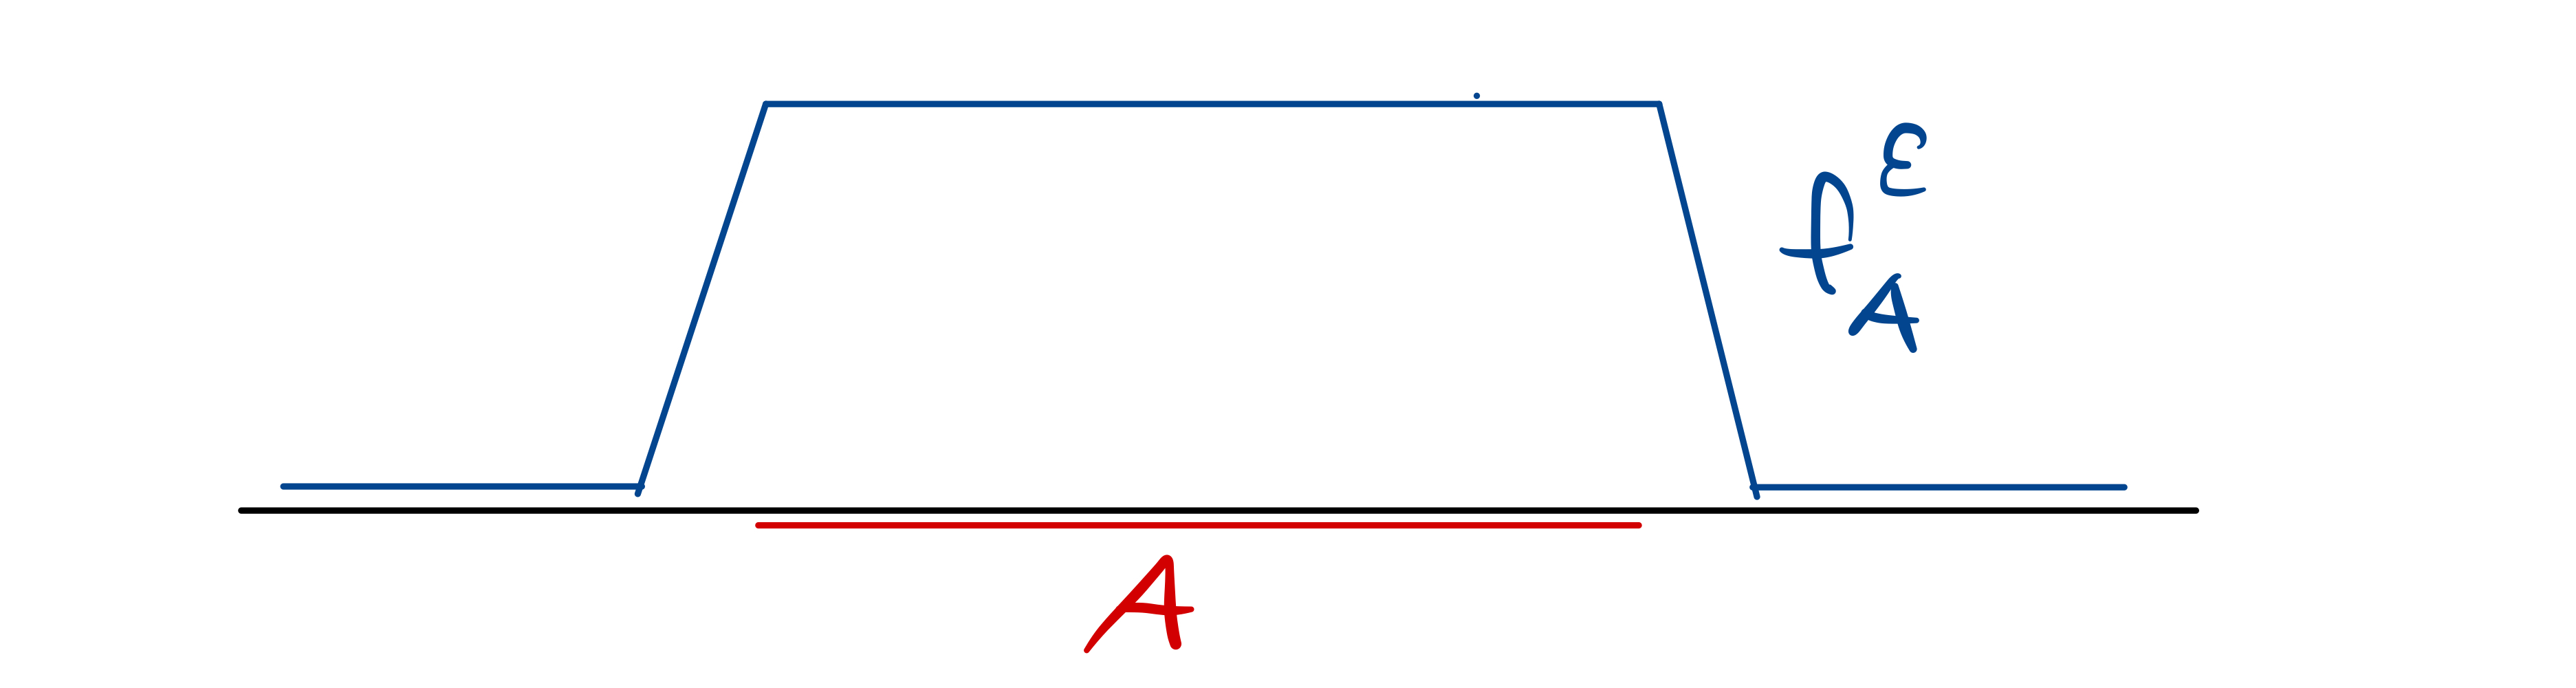
\includegraphics[scale=0.07]{f.jpeg}
			\end{center}
			\vspace{-9mm}
			\end{figure}	
	Remember from basic analysis (or quickly check yourself by using that $\bar A$ are precisely the limits of sequences in $A$) that $d(x,A)=0$ if and only if $x\in \bar A$. The functions $f_A^\varepsilon$ have the following properties:	
			\begin{itemize}
				\item $f_A^{\varepsilon} = 1$ on A
%				\item $f_A^{\varepsilon}(x) = 0$ if $d(x,A)\geq \varepsilon$
				\item $f_A^{\varepsilon} \to \mathbf 1_A$, because for closed sets $d(x,A)=0$ if and only if $x\in A$,
				\item $f_A^{\varepsilon} \leq 1$
			\end{itemize}
			Since the idea of using the functions $f_A^\varepsilon$ is (almost) the entire point of the proof it is useful to check the following yourself:
			\begin{luebung}
				$f_A^{\varepsilon} \in \text{Lip}_{\frac{1}{\varepsilon}}(E)$ and, obviously, $f_A^{\varepsilon} \in C_b(E)$, $f_A^{\varepsilon} \in C_c(E)$.
			\end{luebung}
			We can now use \eqref{Lip} to prove that $\mu$ and $\nu$ coincide on the closed set $A$:
			\begin{align*}
				\mu (A) &= \int_E \mathbf 1_A \dint \mu 
							\overset{\text{DCT}}{=}\lim\limits_{\varepsilon \to \infty} \int_E f_A^{\varepsilon} \dint \mu 
				\overset{\text{ass.}}{=} \lim\limits_{\varepsilon \to \infty} \int_E f_A^{\varepsilon} \dint \nu 
				\overset{\text{DCT}}{=} \int_E \mathbf 1_A \dint \nu = \nu (A).
			\end{align*}
		As explained above we proved that \eqref{Lip} implies $\nu=\mu$, or, in other words, that $\text{Lip}_1(E)$ is separating for $\mathcal M_f(E)$. The claims about $C_b(E)$ and $C_c(E)$ follow in exactly the same way as $f_A^\varepsilon\in C_b(E)$ and $f_A^\varepsilon\in C_c(E)$.
\end{proof}
More explicit classes of functions appear later in the course of this chapter.

\section{Weak convergence of measures - the basics }
As announced the ultimate goal is to prove the convergence of scaled random walks towards the Brownian motion, both seen as function-valued random variables. Let us recall from Definition \ref{Konvergenzarten} the notion of weak convergence of real-valued random variables
\begin{align}\label{weakk}
	\int_\R f \dint \P_{X_n}=\E[f(X_n)]\overset{n\to\infty}{\rightarrow} \E[f(X)]=\int_\R f \dint \P_X,\quad n\to\infty,
\end{align}
which is actually a notion of convergence for the sequence of probability measures $(\P_{X_n})_{n\in\N}$ on $\mathcal B(\R)$. In order define a notion of convergence of stochastic processes we will introduce the law of a stochastic process (or a random variable with general state-space) and then introduce a general notion of weak convergence. 
\begin{ldef}
\begin{deff}
	Let $X$ be a random variable on $(\Omega,\cA,\mathbb{P})$ with values in a metric space $(E,d)$, then \textbf{the law $\mathbb{P}_X$ of $X$} is the probability measure
	\begin{align*}
		\mathbb{P}_X (A) \coloneqq \mathbb{P}\big( X^{-1}(A) \big)= \mathbb{P}\big( \{ \omega \in \Omega \colon  X(\omega) \in A \} \big),\quad A\in \mathcal B(E).
	\end{align*}
	As for real-valued random variables we also use the notion $\mathbb{P}\big( X\in A \big)$ as this can be read more naturally as "{}probability of $X$ in $A$".
\end{deff}
\end{ldef}
For the study of stochastic processes we will always keep in mind the example $E=C([0,1])$ or $E=C([0,\infty))$ which are the state-spaces of stochastic processes indexed by $[0,1)$ or $[0,\infty)$, respectively, reinterpreted as function-valued random variables.\smallskip

In order to speak of convergence of processes we will thus have to define a notion of convergence on measures on more general state-spaces than $\R$. This leads us to the general notion of weak convergence of measures on metric spaces:
\begin{ldef}
\begin{deff}
	Let $(E,d)$ a metric space and $\mu,\mu_1,\mu_2,...\in \mathcal M_f(E)$. We say \textbf{$(\mu_n)_{n\in\mathbb{N}}$ converges weakly to $\mu$} if
	\begin{align*}
		\lim_{n\to\infty} \int_E f\dint \mu_n = \int_E f \dint \mu, \quad \text{for all}\: f \in C_b(E),
	\end{align*}
	and write $\mu_n \overset{\text{(w)}}{\longrightarrow}\mu$ or $\mu_n\Rightarrow \mu$ or $\mu = \operatorname{w-\lim\limits}_{n\to\infty}\mu_n$.
\end{deff}
\end{ldef}
Before returning to probability theory let us discuss important properties that help us to link the general weak convergence theory (a field of Functional Analysis) to properties from Section \ref{sec:konvergenz} in the particular case $E=\R$. 	There are many other ways of defining convergence of measures through distances. They are usually stronger (less sequences converge) which is one of the reasons to speak of weak convergence.
\begin{luebung}
	Let $(\delta_{x_n})_{n\in\N}$ a sequence of Dirac-measures on $E$ such that $x_n\to x$ for $n\to\infty$. Show that $(\delta_{x_n})_{n\in\N}$ converges weakly in $\cM_1(E)$ to $\delta_x$.
\end{luebung}

If you are familiar with Functional Analysis a bit of care is needed as the wording does not match. In the standard terminology of Functional Analysis this is not weak convergence but weak-$*$-convergence on $\cM_f(E)$ using that $\cM_f(E)$ is the dual-space of $C_b(E)$.
\begin{lstep}
\begin{remark}
			If $(E,d)$ is separable then weak convergence in $\cM_f(E)$ can be metrized: Defining the \textbf{\smash{Prohorov metric}} (here the definition for $\nu,\mu\in \cM_1(E)$)
			\begin{align*}
				d_p(\mu,\nu) \coloneqq \inf \big\{ \varepsilon >0 \colon \mu (B) \leq \nu (B_{\varepsilon}(0)) + \varepsilon \:\forall B\in \cB(E) \big\}
			\end{align*}
			one can show that $d_p$ is a metric on $\cM_f(E)$ and
			\begin{align*}
				\mu_n \overset{\text{(w)}}{\longrightarrow}\mu, \: n \to \infty \quad\Leftrightarrow \quad d_p(\mu_n,\mu) \to 0, \: n\to \infty.
			\end{align*}
			This is important as all properties of convergence in  metric spaces (such as uniqueness of limits) hold for weak convergence. Taking $f \equiv 1$ shows that also the total masses must converge. In particular, the weak limit of a sequence of probability measures is a probability measure, no mass gets lost or appears. In other words of topology, $\cM_1(E)$ is a closed subset of $\cM_f(E)$ with respect to the Prohorov metric.

\end{remark}
\end{lstep}
%\begin{example}
%	$\mu_n \coloneqq \delta_{\frac{1}{n}}$, $\mu \coloneqq \delta_0$ are measures in $\mathcal M_f(\mathbb{R})$. Since $$\int_{\mathbb{R}} f \dint \mu_n = f\bigg( \frac{1}{n} \bigg) \overset{n\to \infty}{\longrightarrow} f(0) = \int_{\mathbb{R}} f \dint \mu$$
%	we have $\mu_n \overset{\text{(w)}}{\longrightarrow} \mu$, $n\to\infty$.	
%\end{example}
	\marginpar{\textcolor{red}{Lecture 12}}
We approach weak convergence of measures in two steps. First, we will derive some equivalent conditions, usually referred to Portemantau theorem, via elementary (but tedious) manipulations with measures and integrals. In the next section we start to understand weak convergence from the point of view of convergence in the metric space $(\mathcal M_f,d_P)$ with tools from metric space theory. The metric space approach is necessary in order to derive handy criteria that depend strongly on the corresponding underlying space $(E,d)$.\smallskip

Here is the basic Portemanteau theorem:
\begin{lsatzwichtig}
\begin{theorem}[Portemanteau theorem]
	Let $(E,d)$ a metric space and $\mu,\mu_1,\mu_2,...\in \cM_1(E)$, then the following are equivalent:
	\begin{enumerate}[label=(\roman*)]
		\item $\mu_n \overset{\text{(w)}}{\longrightarrow} \mu,\, n\to\infty$
		\item $\lim_{n\to\infty} \int_E f \dint \mu_n = \int_E f \dint \mu$\:\: $\forall f$ bounded, Lipschitz continuous
		\item $\limsup\limits_{n\to\infty}\mu_n(F) \leq \mu(F) \:\:\: \forall \text{ closed }F\subseteq E$
		\item $\liminf\limits_{n\to\infty}\mu_n(G) \geq \mu(F) \:\:\: \forall \text{ open }G\subseteq E$
		\item $\lim\limits_{n\to\infty}\mu_n(A) = \mu(A) \:\:\:\forall A$ with $\mu(\partial A)=0$
	\end{enumerate}
\end{theorem}
\end{lsatzwichtig}
To understand similarities it is instructive to recall the statment and the proof of Theorem \ref{459} for a sequence $\mu_n=\P_{X_n}$ of probability measures on $\mathcal B(\R)$. In that simpler setting property (v) holds with the closed sets
 $A=(-\infty,t]$ because $\P_X(\{t\})=0$ is equivalent to $t$ being a point of continuity of the distribution function $F_X$. In the next section we will derive a much more useful statement if $(E,d)$ is even a Polish metric space:
 \begin{lwarnhinweis}
	\begin{itemize}
		\item[(vi)] tightness $+$ $\lim_{n\to\infty} \int_E f\dint \mu_n= \int_E f \dint \mu$ for some separating family $C\subseteq C_b(E)$ of $\cM_1(E)$
	\end{itemize}
	\end{lwarnhinweis}
More concrete criteria for special cases such as $E=[a,b], E=[0,\infty)$, $E=\R^d$, or $E=C([0,1])$ will follow below.



\begin{proof}[Proof]

	(i) $\Rightarrow$ (ii): trivial (Lipschitz is continuous)\smallskip
	
	(ii) $\Rightarrow$ (iii): Let $F$ be closed and $f_F^{\varepsilon}$ from the proof of Proposition \ref{theorem_4124}. Then
	\begin{align*}
	 	\limsup\limits_{n\to\infty} \mu_n(F) \overset{\mathbf 1_F\leq f_F^\varepsilon}{\leq} \limsup\limits_{n\to\infty} \int_E f_F^{\varepsilon}\dint \mu_n,\quad \forall \varepsilon >0,
	\end{align*}	
		 so that
	\begin{align*}
		\limsup\limits_{n\to\infty} \mu_n(F) &\leq \inf_{\varepsilon > 0} \limsup\limits_{n\to\infty} \int_E f_F^{\varepsilon} \dint \mu_n \\
		\overset{\text{Limit exists}}&{=} \inf_{\varepsilon > 0} \lim\limits_{n\to\infty} \int_E f_F^{\varepsilon} \dint \mu_n \\
		&= \inf_{\varepsilon > 0} \int_E f_F^{\varepsilon} \dint \mu 
		\overset{\text{DCT}}{=} \mu(F).
	\end{align*}
	
	(iii) $\Leftrightarrow$ (iv): This follows by taking complements as $F$ closed $\Leftrightarrow$ $G = F^c$ open and $\mu_n(F) = 1 - \mu_n(F^c)$ and $\liminf_{n\to\infty}(-a_n) = -\limsup_{n\to\infty}(a_n)$.\smallskip
	
	(iii) $+$ (iv) $\Rightarrow$ (v): Let $A\in \cB(E)$ with $\mu(\partial A) = 0$. First note that 
	\begin{align*}
		 \limsup_{n\to\infty} \mu_n(A) \overset{\text{monot.}}{\leq} \limsup_{n\to\infty} \mu_n({\bar{A}})\overset{\text{(iii)}}{\leq} \mu(\bar{A})
	\end{align*}
	and
	\begin{align*}
		 \liminf_{n\to\infty}\mu_n(A) \overset{\text{monot.}}{\geq} \liminf_{n\to\infty}(\dot{A}) \overset{\text{(iv)}}{\geq}  \mu(\dot{A})
	\end{align*}
	Since $\overline{A} = \dot{A} \cupdot \partial A$ we have $\mu(\dot{A}) + \mu(\partial A) \overset{\text{ass.}}{=} \mu(\bar{A})$ so that $\mu(A)=\mu(\bar A)=\mu(\dot A$) so that the above yields
	\begin{align*}
		 \limsup_{n\to\infty} \mu_n(A)\leq \mu(A) \leq  \liminf_{n\to\infty} \mu_n(A)
	\end{align*}
	which implies that the limit exists and is equal to $\mu(A)$.\smallskip	
	
	(v) $\Rightarrow$ (iii): Let $F \subseteq E$ closed and enlarge $F$ by $\delta$: $F^{\delta}\coloneqq \{ x\in E \,:\, d(x,F) \leq \delta \}$. Since $\partial F^{\delta} \subseteq \{ x\in E \,:\, d(x,E) = \delta \}$ the sets $\partial F^{\delta}$ are disjoint for different $\delta$. Now we use that for a probability measure there cannot be uncountably many disjoint events with positive probability. So there must be a sequence $\delta_k \to 0$ along which $\mu(\partial F^{\delta_k}) = 0$. Hence, we can use (v) for $F^{\delta_k}$ for all $k\in \N$. Thus, 
	\begin{align*}
		\limsup_{n\to\infty}\mu_n(F) \overset{\text{monot.}}{\leq} \limsup_{n\to\infty} \mu_n(F^{\delta_k}) \overset{\text{(v)}}{=}\lim_{n\to\infty}\mu_n(F^{\delta_k}) \overset{\text{(v)}}{=} \mu(F^{\delta_k}),\quad k\in\N,
	\end{align*}
	where we used that limit and limit superior coincide if a limit exists. Now we take limits in $k$ on both sides. Since $F^{\delta_k}\downarrow F$ and the left hand side is independent of $k$, we obtain form monotonicity of measures the desired inequality $\limsup_{n\to\infty}\mu_n(F) \leq \mu(F)$. \smallskip
	
	(iii) $\Rightarrow$ (i): Let $f\in C_b(E)$. Without loss of generality it can be assumed that $0<f<1$. If not, we choose $a>0$ and $b\in\mathbb{R}$ so that $\bar{f} \coloneqq a\cdot f +b \in [0,1)$ and the argument is continued using $\bar f$. Now define the closed sets $F_i^{(k)} \coloneqq \{ x\in E \colon {f}(x) \geq \frac{i}{k} \}$ for $k\in \mathbb{N}, \: 0 \leq i \leq k$. For $\mu \in \cM_1(E)$ monotonicity of integrals and the definition of the integral for simple functions yields
	\begin{align*}
		\sum_{i=1}^k \frac{i-1}{k} \bigg( \mu \big( F_{i-1}^{(k)} \big) - \mu \big(F_i^{(k)}\big)\bigg) \leq \int_E {f}\dint \mu \leq \sum_{i=1}^k \frac{i}{k} \bigg( \mu \big( F_{i-1}^{(k)} \big) - \mu \big(F_i^{(k)}\big)\bigg).
	\end{align*}
	Warning: The inequalities look a bit strange. Typically one would partition the image space $[0,1)$ into the disjoint sets $E^{(k)}_i=\{x \in E \colon \frac{i+1}{k} > {f}(x) \geq \frac{i}{k} \}$ and work with  the inequalities $\sum \frac{i-1}{k} \mu(E_{i-1}^{(k)}) \leq \int_E {f} \dint \mu \leq \sum \frac{i}{k}  \mu(E_{i-1}^{(k)})$, but those sets are not closed. If we use the closed sets $F^{(k)}_i$, then we double count and need to subtract the pieces counted twice. Since $F_k^{(k)} = \emptyset$ and writing out the summand this simplifies to 
	\begin{align*}
		\frac{1}{k} \sum_{i=1}^{k-1} \mu(F_i^{(k)}) \leq \int_E {f}\dint \mu \leq \frac{1}{k} \sum_{i=1}^{k} \mu(F_{i-1}^{(k)}).
	\end{align*}
	This looks more complicated than it is and only comes from looking closely to see the simplifications $\frac{i}{k} \mu ( F_{i-1}^{(k)} )-\frac{i-1}{k} \mu ( F_{i-1}^{(k)})=\frac{1}{k} \mu ( F_{i-1}^{(k)})$ which cancel half of the summands. Note that the estimates also hold for integrals with $\mu_n$ instead of $\mu$, the argument was only based on splitting the function $f$. Using (iii) for the closed sets then gives
	\begin{align*}
		\limsup\limits_{n\to\infty} \int_E {f} \dint \mu_n &\leq \limsup\limits_{n\to\infty} \frac{1}{k} \sum_{i=1}^{k} \mu_n (F_{i-1}^{(k)}) \\
			&\leq \frac{1}{k} \sum_{i=1}^{k} \limsup\limits_{n\to\infty} \mu_n (F_{i-1}^{(k)}) \\
			\overset{\text{(iii)}}&{\leq} \frac{1}{k} \sum_{i=1}^{k} \mu (F_{i-1}^{(k)}) \\
			\overset{ \mu\leq 1 }&{\leq} \frac{1}{k} +\frac{1}{k} \sum_{i=1}^{k-1} \mu (F_{i-1}^{(k)}) \\
			&\leq \frac{1}{k} + \int_E {f} \dint \mu.
	\end{align*}
	Since $k$ was arbitrary, we obtain $\limsup\limits_{n\to\infty} \int_E {f} \dint \mu_n \leq \int_E {f} \dint \mu$. The same reasoning for $-f$ gives $\liminf\limits_{n\to\infty} \int_E  f \dint \mu_n \geq \int_E f \dint \mu$. Both inequalities prove (i).
\end{proof}
For the next theorem recall from Section \ref{sec:push} the notion of the push-forward of a measure under a measurable map. If $g:\Omega \rightarrow \Omega'$ is $(\mathcal A, \mathcal A')$-measurable and $\mu$ is a measures on $\mathcal A$, then we defined $$\mu_g(A):=\mu(g^{-1}(A)),\quad A\in \mathcal A',$$ also written $\mu\circ g$ (more useful if there is a further index), is a measure on $\mathcal A'$. The measure is called the push-forward of $\mu$ under $g$ or the image measure. If we think of converging sequences of measures it is natural to also ask for convergence of the sequence of push-forwards for a given mapping. If $g$ is continuous, this can be proved easily:
\begin{lsatz}
\begin{theorem}[continuous mapping theorem]
	Let $(E_1,d_1)$, $(E_2,d_2)$ be metric spaces and $g\colon E_1 \to E_2$ continuous.
	If $\mu,\mu_1,\mu_2,...$ are finite measures on $\mathcal B(E_1)$, then
	\begin{align*}
		 \mu_n \overset{\text{(w)}}{\rightarrow} \mu,\,\, n\to\infty\quad \Longrightarrow \quad   \mu_n\circ g \overset{\text{(w)}}{\rightarrow} \mu\circ g,\,\, n\to\infty.
	\end{align*}
\end{theorem}
\end{lsatz}
In fact, continuity is not really needed, the assumption $\mu\big( \{ x\in E_1 \,|\, g \:\text{not continuous in }x \}\big) = 0$ is enough for the theorem to hold, but the proof is a bit lengthy.
\begin{proof}[Proof]
 Let $f\in C_b(E_2)$, then $f\circ g \in C_b(E_1)$. Using the transformation formula for integrals twice (see Theorem \ref{trafo}) then gives
\begin{align*}
	\int_{E_2}f\dint \mu_n \circ g = \int_{E_1} f\circ g \dint \mu_n \overset{n\to\infty}{\longrightarrow} \int_{E_1}f\circ g \dint \mu  = \int_{E_2} f\dint \mu \circ g.
\end{align*}
Hence, $\mu_n \circ g \overset{\text{(w)}}{\rightarrow} \mu \circ g$.
\end{proof}
% CMT
%\begin{lsatzwichtig}
%\begin{theorem}[continuous mapping theorem]
%	Let $(E_1,d_1)$, $(E_2,d_2)$ be metric spaces and $\varphi\colon E_1 \to E_2$ Borel-measurable.
%	If $\mu,\mu_1,\mu_2,...\in M_1(E_1)$ and $\mu\big( \{ x\in E_1 \,|\, \varphi \:\text{not continuous in }x \}\big) = 0$ then
%	\begin{align*}
%		\mu = \text{w-}\lim\limits_{n\to\infty} \mu_n \:\: \Rightarrow \:\: \mu \circ\varphi = \text{w-}\lim\limits_{n\to\infty} \mu_n \circ \varphi
%	\end{align*}
%\end{theorem}
%\footnote{Leif: Do we need this general version?}
%\end{lsatzwichtig}
%Important special case: $\varphi$ continuous. \\%
%Easy proof: Let $f\in C_b(E_2)$, then $f\circ \varphi \in C_b(E_1)$. Trafo-formula yields
%\begin{align*}
%	\int_{E_2}f\dint \mu_n \circ \varphi = \int_{E_1} f\circ \varphi \dint \mu_n \overset{n\to\infty}{\longrightarrow} \int_{E_1}f\circ \varphi \dint \mu  = \int_{E_2} f\dint \mu \circ \varphi
%\end{align*}
%Hence, $\mu_n \circ \varphi \overset{\text{(w)}}{\Rightarrow} \mu \circ \varphi$.
%\begin{proof}[Proof]
%	Without continuity we need Portemanteau and a bit of topology.
%	\begin{enumerate}[label=(\roman*)]
%		\item
%			Claim: $U_{\varphi} \coloneqq \{ x\in E_1 \,|\, \varphi \text{ not continuous in x } \} \in \cB(E_1)$
%			Why?\\
%			Define $$ A_{m,n} \coloneqq \{ x \in E_1 \,|\, \exists y,z \in \cB_{\frac{1}{m}}(x) \text{ with } d_2 \big(\varphi(y),\varphi(z) \big) > \frac{1}{n} \}$$
%			$A_{m,n}$ is open ($\bigtriangleup$-inequality), hence $A \in \cB(E)$. But then ($\varepsilon$-$\delta$-definition of continuity)
%			$$ U_{ \varphi} = \bigcup_{n\in\mathbb{N}}\bigcap_{m\in\mathbb{N}} A_{n,m} \in \cB(E_1)$$
%		\item
%			We use (iii) from Portemanteau: \\
%			Suppose $F \subseteq E_2$ is closed. Then
%			\begin{align*}
%				\limsup_{n\to\infty} \mu_n \big( \varphi^{-1} ( F ) \big) \overset{\text{mon.}}{\leq} \limsup_{n\to\infty} \mu_n \big( \underbrace{ \overline{\varphi^{-1} ( F )}}_{\text{closed}} \big) \leq \mu \big( \varphi^{-1} ( F ) \big)
%			\end{align*}
%			Next we show $\overline{\varphi^{-1} ( F )} \overset{\star}{\subseteq} ( \varphi^{-1} ( F ) \cup U_{\varphi}$ , hence $\mu \big( \overline{\varphi^{-1} ( F )} \big) = \mu \big(  \varphi^{-1} ( F ) \big)$ due to $\mu(U_{\varphi} ) = 0$ by assumption. Combining the aboce we get
%			\begin{align*}
%				\limsup_{n\to\infty} \mu_n \circ \varphi (F) \leq \mu \circ \varphi (F)
%			\end{align*}
%			for all $F \subseteq E_2$ closed and again from Portemanteau we obtain $\mu_n \circ \varphi \overset{\text{(w)}}{\longrightarrow} \mu \circ \varphi$, $n\to\infty$.\\
%			Why does $\star$ hold? We only need to show $\partial \varphi^{-1}(F) \subseteq \varphi^{-1}(\partial F ) \cup U_{\varphi}$. Recall: If $\varphi$ is continuous in $x$, then $\forall \delta > 0 \exists > 0: \varphi \big( B_{\varepsilon}(x) \big) \subseteq B_{\delta}(\varphi(x))$.
%			\begin{itemize}
%				\item
%					If $x \in \partial \varphi^{-1}(F)$ and $\varphi$ is not continuous in $x$, then $x\in U_{\varphi}$.
%				\item
%					If $x \in \partial \varphi^{-1}(F)$ and $\varphi$ is continuous in $x$, then take $\varepsilon,\delta$ from above. There are $y\in \varphi^{-1}(F)\cap B_{\varepsilon}(x)$ and also $z \in \varphi^{-1}(F^C)\cap B_{\varepsilon}(x)$. Therefore, $\varphi(y) \in F\cap B_{\delta}\big(\varphi(x)\big)$ and $\varphi(z) \in F^C \cap B_{\delta}\big(\varphi(x)\big)$. Hence, $\varphi(z)\in \partial F$.
%			\end{itemize}
%	\end{enumerate}
%\end{proof}
We finish the section by writing down the generalised notion of convergence that was announced at the beginning of this section:
\begin{ldef}
\begin{deff}
	Let $X, X_1, X_2,...$ be random variables with values in a metric space $(E,d)$. Then we say that \textbf{$(X_n)_{n\in\N}$ converges to $X$ in distribution} if $\mathbb{P}_{X_n} \overset{\text{(w)}}{\longrightarrow} \mathbb{P}_{X}$, $n\to \infty$. One usually writes $X_n\overset{\text{(d)}}{\to} X$, $X_n \Rightarrow X$ or $X_n \Rightarrow \mathbb{P}_X$ for $n\to\infty$ and also says $(X_n)_{n\in\N}$ converges weakly to $X$. 
\end{deff}
\end{ldef}
Realising that $f(X_n)$ is a real-valued random variable we find that convergence in distribution can be rewritten in the more probabilistic language 
\begin{align*}
	X_n \overset{\text{(d)}}{\longrightarrow}X,\: n\to\infty\quad  \Leftrightarrow\quad \lim_{n\to\infty} \E[f(X_n)]= \E[f(X)],\quad \forall f\in C_b(E).
\end{align*}


In the case of real-valued random variables this is nothing else but the convergence in distribution from \eqref{weakk} that was used to formulate the central limit theorem. This also explains why sometimes convergence in distribution of random variables is called weak convergence. For random variables the continuous mapping theorem states
\begin{align*}
	X_n\overset{\text{(d)}}{\longrightarrow} X,\,\,n\to\infty\quad \Longrightarrow\quad g(X_n)\overset{\text{(d)}}{\longrightarrow} g(X),\,\,,n\to\infty
\end{align*}
for all continuous $g$, a statement that is used a lot!\smallskip

We will now turn towards the study of weak convergence of measures seen as metric convergence in $(\cM_f(E),d_P)$ which is based on the following characterisation of convergence:
\begin{lsatzwichtig}
\begin{prop}\label{propkonvergenz}
	Let $(E,d)$ a metric space and $(x_n)_{n\in\N}$ a sequence in $E$. Then the following are equivalent:
	\begin{itemize}
		\item $x_n\to x, n\to\infty,$
		\item 
		\begin{enumerate}[label=(\roman*)]
			\item $A:=\{x_n:n\in\N\}$ is relatively sequentially compact.
			\item $x_{n_k}\to x,k\to\infty,$ for all converging subsequences.
		\end{enumerate}
	\end{itemize}
\end{prop}
\end{lsatzwichtig}
\begin{proof}[Proof]
	"$\Rightarrow$": Any subsequences of converging sequences converge to the same limit, hence, the second limit follows trivially and also the relative sequential compactness follows.\smallskip
	
	"$\Leftarrow$": If $(x_n)$ does not converge towards $x$ then there is some $\varepsilon>0$ and a subsequence with $d(x_{n_k},x)>\varepsilon$. Since also the subsequence $(x_{n_k})\subseteq (x_n)$ is relatively sequentially compact there is another subsequence $(x_{n_k'})$ of $(x_{n_k})$ that converges. Since the limit must be $x$ by assumption we find $d(x_{n_k'},x)<\varepsilon$ for $k$ large enough. But this is a contradiction.
\end{proof}
In order to use the proposition for weak convergence of measures we will proceed in three steps. In Section \ref{sec:tight} a characteristation of relative sequential compactness will be proved. The so-called tightness gives a condition that can be checked if compact sets of $E$ are sufficiently well understood. Section \ref{sec:unique} adresses the problem of identifying limits of subsequences. Finally, combining both sections we can derive good conditions for convergence of measures on different Polish spaces $(E,d)$. 


 %For real-valued random  variables the continuous mapping theorems only states that
%\begin{align*}
%	X_n \overset{\text{(d)}}{\longrightarrow}X,\: n\to \infty \quad \Longrightarrow \quad g(X_n) \overset{\text{(d)}}{\longrightarrow} g (X), \: n \to \infty,
%\end{align*}
%for all continuous $g$ which of course follows trivially from the definition of weak convergence as for all $f\in C_b$ also $f\circ g \in C_b$.
	\marginpar{\textcolor{red}{Lecture 13}}

\section[Relative sequential compacteness of measures]{Relative sequential compacteness of measures}\label{sec:tight}




In the light of Proposition \ref{propkonvergenz}. The aim of this section is to derive a well accessible equivalent notion to relative sequential compactness in this particular metric space. 

\begin{ldef}
\begin{deff}\label{def_tight}
	A family $\cF \subseteq \cM_f(E)$ is called \textbf{tight}  if for every $\varepsilon>0$ there is a compact set $K \subseteq E$ with $$ \sup_{\mu \in \cF} \mu \big(K^c\big) < \varepsilon$$
\end{deff}
\end{ldef}
To get a visual idea of tightness recall the interpretation of a measure that describes how mass is distributed over the state-space $E$. Tightness means that no mass gets lost towards infinity, the mass of all measures is (uniformly) concentrated in compact sets. 
\begin{figure}[h]
			\begin{center}
				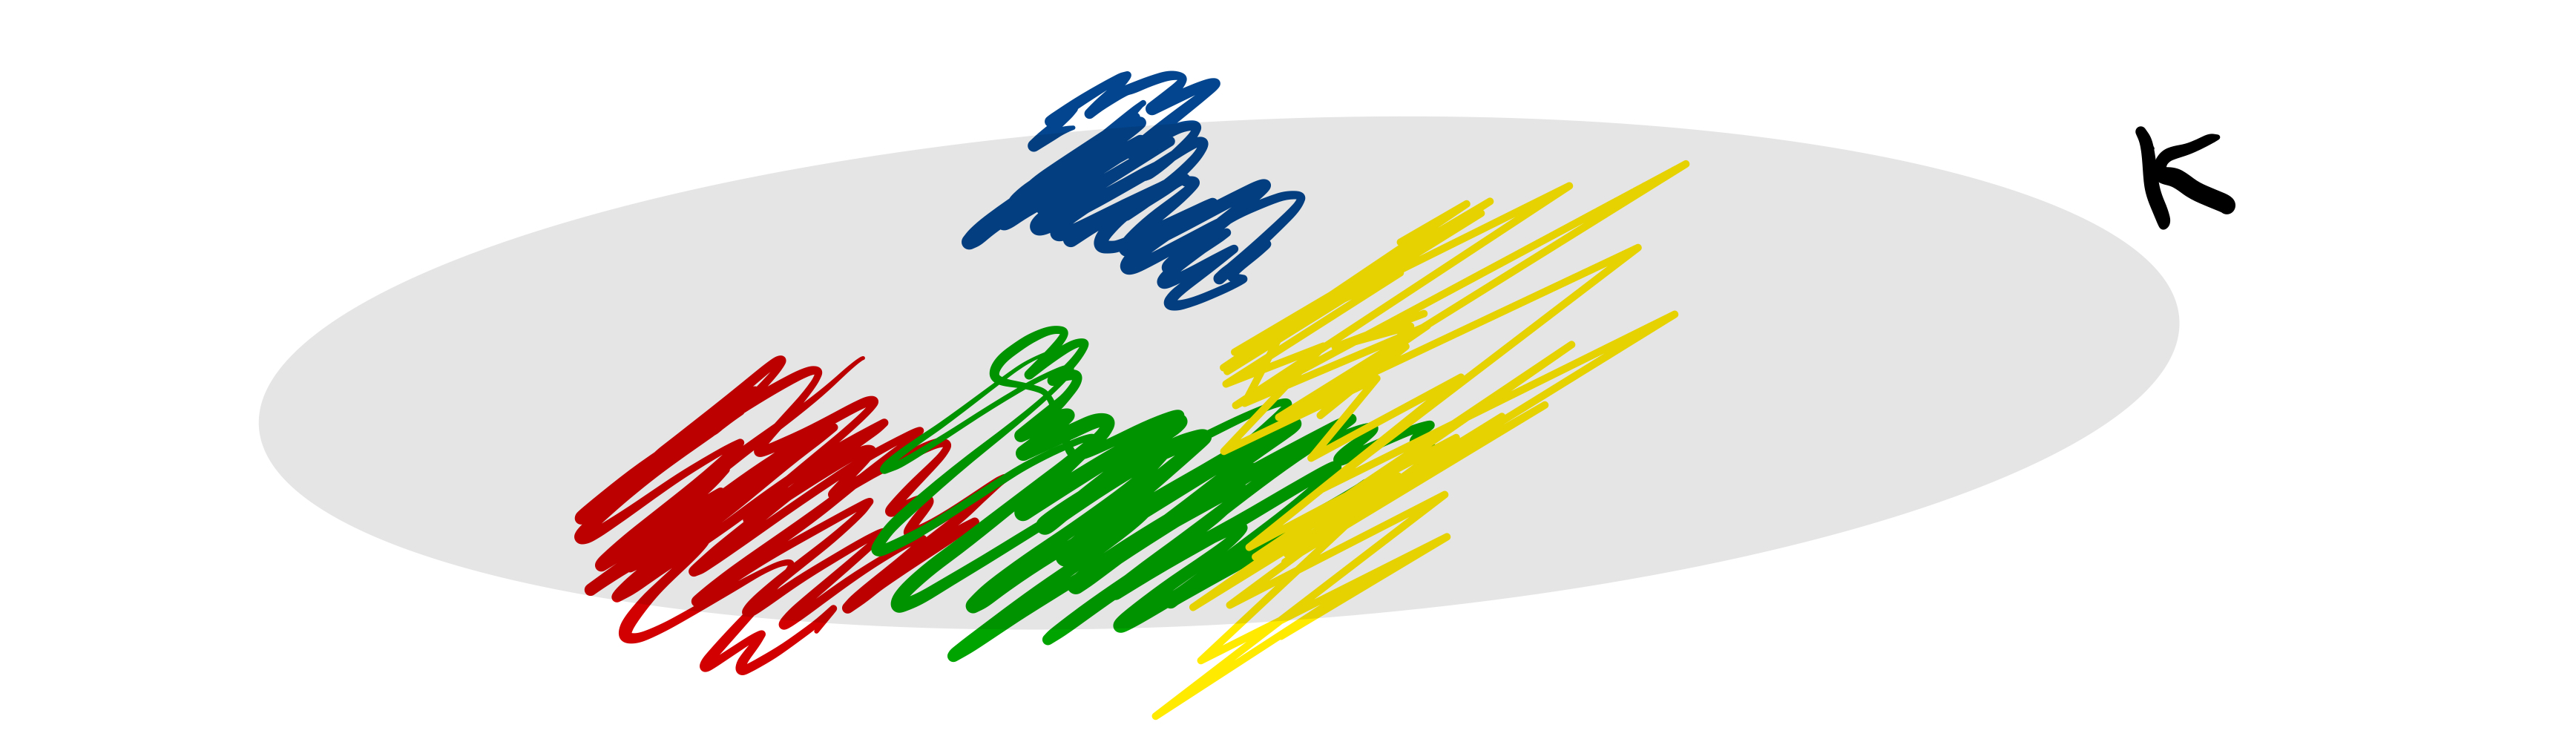
\includegraphics[scale=0.07]{tight.jpeg}
			\end{center}
			\vspace{-7mm}
			\caption*{Tightness of four measures visualised in terms of distribution of mass}
			\end{figure}
			Before we go into Prohorov's theorem let us check some examples to get some feeling of tight families.

\begin{example}
	\begin{itemize}
		\item
			By Proposition \ref{prop_4120} every family consisting of a single measure on a Polish space is tight
		\item
			$(\delta_{x_n})_{n\in\mathbb{N}}$ is a tight sequence for a Polish space $(E,d)$ if and only if $(x_n)_{n\in\N}$ is totally bounded in $E$. For instance if $(x_n)_{n\in\N}$ is bounded for $E=\R$.
		\item
			If a family $(X_\alpha)_{\alpha\in I}$ of real-valued random variables is bounded in $L^1$, then the family of the laws $\{ \mathbb{P}_{X_\alpha} \colon \alpha\in I \}$ is tight. This follows from our beloved Markov inequality as follows. If $C$ is the $L^1$-bound and $\varepsilon>0$, then $K:=[-C/\varepsilon, C/\varepsilon]$ does the job:
			\begin{align*}
				\mathbb{P}_{X_\alpha}(K^c)
				= \mathbb{P}\big(\lvert X_\alpha \rvert > C/\varepsilon\big) \overset{\text{Markov}}{\leq} \frac{\E[\lvert X_\alpha \rvert ]}{C/\varepsilon} \leq \varepsilon
			\end{align*}
		\item
			$\{ U([-n,n])\colon n\in \mathbb{N} \}$ is not tight in $\cM_f(\mathbb{R})$ as mass disappears towards infinity.
					\item If $K$ is a compact set and $(\mu_n)_{n\in\N}$ is a sequence in $\cM_1(E)$ with $\mu_n(K)=1$ for all $n\in\N$, then $(\mu_n)_{n\in\N}$ is tight.
	\end{itemize}
\end{example}
The final example shows that a good understanding of compact sets of $E$ can be extremely useful to understand tightness. We will return to this observation once we discuss in more detail $E=C([0,1])$ in which for instance sets of bounded H\"older continuous functions are compact.\smallskip

The importance of tightness becomes clear with Prohorov's famous theorem in combination with Proposition \ref{propkonvergenz}.
\begin{lsatz}
\begin{theorem}[Prohorov]\label{Prohorov}
	Let $(E,d)$ be a Polish metric space and $\cF \subseteq \cM_1(E)$, then
	\begin{align*}
		 \cF \text{ is weakly relatively sequentially compact}\quad \Leftrightarrow \quad \cF \text{ is tight}.
	\end{align*}
\end{theorem}
\end{lsatz}
The formulation of Prohorov's theorem is frightening on first sight, weakly relatively sequentially compact means that the subset $\cF$ of $\mathcal M_1(E)$ is relatively compact (the closure is compact) with respect to the topology induced by the Prohorov metric. Using properties of closures and the sequential compactness this means that every sequence $(\mu_n)$ in $\cF$ has a subsequence that converges to some limit in $\cM_f$ but the limit does not necessarily belong to $\cF$. The entire point is that Prohorov's theroem connects a measure property (tightness) with a topological property (compactness).
\begin{proof}[Proof]
	There is a relatively simple and a very hard direction. We start with the simpler one and discuss the hard direction only for $E=\R$. A sketch for the general case is given after the proof.\\
	
	"{}$\Leftarrow$": We start with arguments similar to the ones from the proof of Proposition \ref{prop_4120}. Let $x_1,x_2,...$ be dense in $E$ and 
	\begin{align*}
		A_{N,n} \coloneqq \bigcup_{k=1}^N B_{\frac{1}{n}}(x_k) \:\: \uparrow E,\quad N\to\infty.
	\end{align*}
	We first prove that
	\begin{align}\label{eq_4_1}
		\lim\limits_{N\to\infty} \inf\limits_{\mu\in\cF} \mu (A_{n,N}) =1, \quad \forall n\in\mathbb{N}.
	\end{align}
	Suppose \eqref{eq_4_1} does not hold for some $n\in\N$. Then there is some $c<1$, an increasing sequence $(N_j)$ of natural numbers and a sequence of measures $\mu_j \in \cF$ with $$\lim_{j\to\infty} \mu_j (A_{n,N_j}) \leq c < 1.$$ Since the sequence is weakly relative sequentially compact there is a subsequence $(\mu_{j_k})$ that converges to some $\mu \in \cM_1(E)$ (not necessarily in $\cF$, $\mu$ could be in $\bar{\cF}$). Since the $A_{n,N}$ are open, Portemanteau gives for all $N$
	\begin{align*}
		\mu(A_{n,N}) \leq \limsup_{k\to\infty}\mu_{j_k}(A_{n,N}) 
			\overset{\text{mon.}}{\leq} \limsup_{k\to\infty} \mu_{j_k}(A_{n,N_{j_k}}) 
			\leq c < 1.
	\end{align*}
	But this gives a contradiction: $1 = \mu(E) \overset{\text{cont.}}{=} \lim_{k\to\infty} \mu (A_{n,N_{j_k}}) \leq c<1$. \smallskip
	
	Now we use \eqref{eq_4_1} to deduce the tightness. There are $N,n_N$ with $\mu(A_{n_N,N}) \geq 1 - \frac{\varepsilon}{2^N}$ for all $\mu \in \cF$. Defining $K \coloneqq \bigcap_{N=1}^{\infty} \bar{A}_{n_N,N}$, $K$ is closed and totally bounded, hence, $K$ is compact as $E$ is complete. Additionally,
	\begin{align*}
		\mu(K^c) &= \mu \Big( \bigcup_{N=1}^{\infty} \bar{A}_{n_N,N}^c \Big) \\
			\overset{\text{sub. add.}}&{\leq} \sum_{N=1}^{\infty} \mu ( \bar{A}_{n_N,N}^c) \\
			&= \sum_{N=1}^{\infty} \big( 1 - \mu (\bar{A}_{n_N,N}) \big) \\
			\overset{\text{mon.}}&{\leq} \sum_{N=1}^{\infty} \big( 1 - \mu (A_{n_N,N}) \big) \leq \varepsilon
	\end{align*}
	for all $\mu \in \cF$. Hence, $\cF$ is tight.\smallskip
	
	"{}$\Rightarrow$": Considering only $E=\R$ we have the big advantage that one can argue using the cumulative distribution function since $$ \mu_n \overset{\text{(w)}}{\longrightarrow}\mu, \: n \to \infty \quad \Leftrightarrow \quad F_{\mu_n}(t) \to F_{\mu}(t), \: n\to\infty$$ for all points of continuity of $F$. Recall Theorem \ref{459} and keep in mind that convergence in distribution of a sequence of random variables $X_n\sim F_n$ is equivalent to weak convergence of the corresponding sequence of probability measures $\P_{F_n}$. Here we use the measures $\mu_n$ and denote the corresponding CDFs by $F_n \coloneqq \mu_n\big( ( -\infty,t]\big)$, $t\in \mathbb{R}$. Reformulated this way, Prohorov's theorem is only a theorem on CDFs: Every tight sequence of probability measures has a subsequence for which the CDFs converge to a limiting CDF at all points of continuity.\smallskip
	
	Let $(\mu_n)_{n\in\mathbb{N}}$ be a sequence in $\cF$ and $(F_n)_{n\in \mathbb{N}}$ the corresponding sequence of CDFs. Since $\big( F_n(t)\big)_{n\in\mathbb{N}}$ is bounded for all $t\in\R$ there is a convergent subsequence. Using diagonalisation \footnote{explain} there is a subsequence $(n_k)_{k\in\mathbb{N}}$ so that $F_{n_k}(q) \to \tilde{F}(q)$, $q\in\mathbb{Q}$, for some function $\tilde{F}$. We will check that
	\begin{enumerate}[label=(\roman*)]
		\item
			$F(t) \coloneqq \inf \big\{ \tilde{F}(q) \colon q > t, \: q\in \mathbb{Q}\big\}$, $t\in\R$, is a cumulative distribution function.
		\item
			$\mu_n \overset{\text{(w)}}{\longrightarrow} \mu,\,n\to\infty$, where $\mu\sim F$.
	\end{enumerate}
	Both claims are mostly technical and not too surprising, the interesting point is how the tightness comes in. The tightness is needed to prove that $F$ does not loose mass at infinity, i.e. $\lim_{t\to+\infty} F(t)=1$.
	\begin{enumerate}[label=(\roman*)]
		\item Let us check the defining properties of a cumulative distribution function. We are a bit sloppy for the claims that obviously hold even though writing the details is a bit tedious (playing with $\varepsilon$-$N$ and the definition of the infimum), those details do not lead to any deeper understanding. We actually skipped the same arguments before in the proof of Theorem \ref{kernel}.
			\begin{itemize}
				\item $F\colon \:\mathbb{R} \to [0,1]$, since $F_n \colon \mathbb{R}\to [0,1]$.
				\item $\tilde{F}$ is increasing on $\mathbb{Q}$ as all $F_n$ are increasing, then $F$ inherits the property construction.
				\item $F$ is right-continuous by definition (here one should work careful with the definition of the infimum).
				\item $\lim_{t\to+\infty}F(t) = 1$, $\lim_{t \to-\infty}F(t) = 0$ is the interesting part. This is tightness, no mass gets lost. The implications look complicated but the argument is simple:
					\begin{align*}
						\text{Tightness } \quad 
						&\Rightarrow\quad \forall \varepsilon > 0 \,\exists M\in \Q\colon \mu \big( [ -M,+M]^c \big) < \varepsilon \:\: \forall \mu \in \cF \\
						&\Rightarrow\quad \forall \varepsilon > 0 \,\exists M\in \Q\colon \mu_n \big( [ -M,+M]^c \big) < \varepsilon \:\: \forall n\in\N\\
									&\Rightarrow\quad \forall \varepsilon > 0\, \exists M\in \Q\colon 1-F_n(M)+F_n(-M) < \varepsilon \:\: \forall n \in \mathbb{N} \\
												&\Rightarrow\quad \forall \varepsilon > 0 \,\exists M\in\Q \colon F_n(M) \geq 1- \varepsilon, F_n(-M)\leq \varepsilon \:\: \forall n \in \mathbb{N} \\
												&\Rightarrow\quad \forall \varepsilon > 0 \,\exists M\in \Q\colon F(M) \geq 1- \varepsilon, F(-M)\leq \varepsilon \\
												&\Rightarrow\quad \lim_{t\to+\infty} F(t) = 1, \lim_{t\to-\infty}F(t)=0.
					\end{align*}
			\end{itemize}
		\item As explained above we can apply Theorem \ref{459} and prove the pointwise convergence of the CDFs $F_n$ at all points of continuity of $F$. Let $t$ be a point of continuity and $\varepsilon>0$. \footnote{Bild}
			Then there are $q_i \in \mathbb{Q}$ with $q_1 < q_2 < t < q_3$ with $F(q_3) - F(q_1) < \varepsilon$. Using monotonicity we have
			\begin{align*}
				F_{n_k}(q_2) \leq F_{n_k}(t) \leq F_{n_k}(q_3),
			\end{align*}
			which gives
			\begin{align*}
				\tilde F(q_2)=\liminf F_{n_k}(q_2) \leq \liminf F_{n_k}(t) \leq \limsup F_{n_k}(t) \leq \limsup F_{n_k}(q_3)=\tilde F(q_3)
			\end{align*}
			using the convergence on $\Q$. Hence,
			\begin{align*}
				F(q_1) \leq \tilde{F}(q_2) \leq \liminf F_{n_k}(t) \leq \limsup F_{n_k}(t) \leq \tilde{F}(q_3) \leq F(q_3).
			\end{align*}
			But this implies that 
			\begin{align*}
				 \liminf F_{n_k}(t),  \limsup F_{n_k}(t)\in [F(t)-\varepsilon, F(t)+\varepsilon].
			\end{align*}
			Since $\varepsilon$ is arbitrary we proved that $\lim F_{n_k}(t)$ exists and is equal to $F(x)$. 
	\end{enumerate}
\end{proof}
Here is a sketch on how the complicated "{}$\Rightarrow$"{} direction of Prohorov's theorem is proved for general Polish spaces:
\begin{enumerate}[label=(\roman*)]
	\item
		Since $E$ is separable there is a countable base $\cU \subseteq \tau$ for the topology, i.e. $O = \bigcup\limits_{U\in\cU, U \subseteq O} U$ for all $O$ open.
	\item
		Define a possible limit measure on $\cU\colon$ $\big( \mu_n(U)\big)_{n\in\mathbb{N}}$ is a bounded sequence, hence, has a converging subsequence. Since there are countably many $U_1$, $U_2$,$....\in\cU$ the same diagonalisation argument gives a subsequence such that $\big( \mu_{n_k}(U) \big)_{k\in\mathbb{N}}$ converges for all $U$.
	\item
		Define $\mu(U) \coloneqq \lim_{k\to\infty} \mu_{n_k}(U)$ for all $U \in \cU$.
	\item
		Main step: Carath\'{e}odory extension style construction of a probability measure $\bar{\mu}$ on $\cB(E)$ with $\bar{\mu}(U) = \mu(U)$ for all $U\in \cU$.
	\item
		Show $\bar{\mu}(O) \leq \liminf_{k\to\infty} \mu_{n_k}(O)$ for all $O$ open.
	\item Portemanteau implies $\mu_{n_k} \overset{\text{(w)}}{\longrightarrow} \mu$, $k\to\infty$.
\end{enumerate}
Hence, there is a weakly converging subsequence (not necessarily to a limit in $\mathcal F$) and this is precisely the relative compactness with respect to weak convergence.\smallskip

A first simple consequence of Prohorov's characterisation is the following reformulation of Proposition \ref{propkonvergenz} for weak convergence of probability measures:
\begin{lsatz}
\begin{prop}[A useful characterization of weak convergence]\label{most_useful_characterization_weak_convergence}
	Let $(E,d)$ be a Polish metric space and $\mu,\mu_1$, $\mu_2$,$...\in \cM_1(E)$. Then weak convergence of $\mu_n$ to $\mu$ is equivalent to
	\begin{enumerate}[label=(\roman*)]
			\item $\{\mu_n:n\in\N\}$ is tight,
			\item $ \lim_{n\to\infty} \int_E f \dint \mu_n = \int_E f \dint \mu$ for \underline{some} separating family $C \subseteq C_b(E)$ of $\cM_1(E)$.
		\end{enumerate}
\end{prop}
\end{lsatz}
\begin{proof}[Proof]
	"{}$\Rightarrow$": Converging sequences are relatively compact sets (in metric spaces all subsequences have the same limit), hence, tight by Prohorov's theorem. The convergence of the integrals holds by definition of weak convergence (even for all $f\in C_b(E)$).\smallskip	
	
	
	"{}$\Leftarrow$": We use Proposition \ref{propkonvergenz}. Tightness implies the sequential relative compacteness and we only need to identify $\mu$ as limit of all converging subsequences. If $(\mu_{n_k})$ is a subsequences of $(\mu_n)$ with limit $\nu$, then
\begin{align*}
	\int_E f \dint \mu=\lim_{n\to\infty} \int_E f \dint \mu_{n}=\lim_{k\to\infty} \int_E f \dint \mu_{n_k'}=\int_E f \dint \nu,\quad f\in C.
\end{align*}
The first equality holds for all $f\in C$ by assumption, the second as $(\mu_{n_k})$ is a subsequence, and the third even for all $f\in C_b(E)$. Since $C$ was assumed to be separating we proved $\nu=\mu$. 
%
%	
%	
%	Let's assume that $\mu_n$ does not converge weakly towards $\mu$. Then there is some $h\in C_b(E)$ with $$ \int_E h \dint \mu_n \not\to \int_E h \dint \mu,\quad n \to \infty$$
%	Then there is some $\varepsilon > 0$ and a subsequence $(n_k)_{k\in\mathbb{N}}$ with 
%	\begin{align}\label{eq_4_2}
%		\bigg\lvert \int_E h \dint \mu_{n_k} - \int_E h \dint \mu \bigg\rvert > \varepsilon,\quad \forall k \in \mathbb{N}.
%	\end{align}
%	Since $(\mu_{n_k})_{k\in\mathbb{N}}$ is also tight, by Prohorov's theorem there is a subsequence $(n_{k^{\prime}})_{k\in\mathbb{N}}$ of $(n_k)_{k\in\mathbb{N}}$ and a measure $\nu\in \cM_1(E)$ with $\mu_{n_{k^{\prime}}} \overset{\text{(w)}}{\longrightarrow} \nu$, hence, $$\int_E h \dint \mu_{n_{k^{\prime}}} \to \int_E h \dint \nu.$$
%	Since \eqref{eq_4_2} also holds for the subsequence we get $\int_E h \dint \mu \neq \int_E h \dint \nu$. On the other hand, by assumption, for all $f\in C_b(E)$,
%	\begin{align*}
%		\int_E f \dint \mu \overset{\mu_{n_{k^{\prime}}} \overset{\text{(w)}}{\longrightarrow} \mu}{=}\lim_{n\to\infty} \int_E f \dint \mu_{n_{k^{\prime}}} \overset{\mu_{n_{k^{\prime}}} \overset{\text{(w)}}{\longrightarrow} \nu}{=} \int_E f \dint \nu
%	\end{align*}
%	which implies $\mu = \nu$ since $C$ is a separating family. 
\end{proof}
%The next sections will deal with the prime examples that are needed for applications in probability: $(\R,|\cdot |)$ and $(\R^d,|\cdot |)$ for real-valued random variables and random vectors, $( C( [ 0, 1 ] \big), ||\cdot ||_\infty)$  and $( C( [ 0, \infty ) \big), ||\cdot ||_\infty)$ for stochastic processes.

In order to prove weak convergence we will often refer to Proposition \ref{most_useful_characterization_weak_convergence}, but there are two drawbacks that depend crucially on the underlying space $E$. One needs a good understanding of tightness (i.e. of compact sets of $E$) and one needs a good separating family. For instance for $E=C([0,1])$ it will turn out to be more useful to circumvent the formulation of Proposition \ref{most_useful_characterization_weak_convergence} and argue a bit more directly.

% !TeX spellcheck = en_US
%\chapter{Characteristic Functions and the Central Limit Theorem}
	\marginpar{\textcolor{red}{Lecture 14}}
\section[Identification of probability laws on $\R$]{Identification of probability laws on $\R^d$}\label{sec:unique}
The previous section showed how to reformulate relative sequential compactness in terms of tightness. In this section we will deal more closely with the second property from Proposition \ref{propkonvergenz}, the identification of limits of converging subsequences. We will give precise examples that help to apply Proposition \ref{most_useful_characterization_weak_convergence} for particularly simple $E$. As a side product we derive ways of determining the law of a random variable through "{}enough"{} expectations. Before doing so let us dive a bit into approximation theory.
\begin{lsatzwichtig}
\begin{theorem}[Weierstra\ss{} approximation theorem]\label{Weierstrass_approx}
	Let $f \colon [0,1] \to \mathbb{R}$ be continuous, then there is a sequence $(f_n)_{n\in\mathbb{N}}$ of polynomials on $[0,1]$ with $\left\Vert f_n - f \right\Vert_{\infty} \to 0, \: n \to \infty$.\smallskip
	
	In words: The polynomials are dense in $( C([0,1]),||\cdot||_\infty)$.
\end{theorem}
\end{lsatzwichtig}
The proof we give is awesome, as it is a probabilistic proof for an analytic theorem. The sequence of polynomials is actually given explicitly, the so-called Bernstein polynomials.
\begin{proof}[Proof]
	Let $X_1,...,X_n$ be iid Ber$(p)$-distributed random variables, hence, $S_n = \sum_{k=1}^n X_k$ is $\text{Bin}(n,p)$-distributed. Now recall the proof of the weak law of large numbers \eqref{schwaches} - Tschebycheff and Bienaymé:
	\begin{align*}
		\mathbb{P}\Big( \Big| \frac{S_n}{n}-p \Big| > \varepsilon \Big) \leq \frac{\mathbb{V}(S_n)}{n^2 \varepsilon^2} = \frac{n\V[X_1]}{n^2 \varepsilon^2} = \frac{p(1-p)}{n \varepsilon^2}
	\end{align*}
	Next, computing the discrete expectation for $\text{Bin}(n,p)$ yields
	\begin{align*}
		\E \Big[ f \Big( \frac{S_n}{n} \Big) \Big] = \sum_{k=0}^n f \Big(\frac{k}{n}\Big){n\choose k} p^k (q-p)^{n-k} = f_n(p)
	\end{align*}
	with the so-called Bernstein polynomial
		$$f_n(x) =  \sum_{k=0}^n  f \Big(\frac{k}{n}\Big){n\choose k} x^k (1-x)^{n-k},\:\: x\in [0,1].$$
	Now fix $\varepsilon > 0$. Since $f$ is uniformly continuous ($[0,1]$ is compact) there is some $\delta>0$ with
		\begin{align*}
			\lvert x - x^{\prime} \rvert < \delta \: \Rightarrow \: \lvert f(x) - f(x^{\prime}) \rvert < \varepsilon,
		\end{align*}
		so that we can estimate 
		\begin{align*}
			\Big| f \Big( \frac{S_n}{n} \Big) - f(p) \Big| \leq \varepsilon + \mathbf 1_{\lvert \frac{S_n}{n}-p \rvert \geq \delta} 2  \left\Vert f \right\Vert_{\infty}.
		\end{align*}	
		This gives
		\begin{align*}
			\lvert f_n(p) - f(p) \rvert &= \Big| \E \Big[ f \big( \frac{S_n}{n} \big) \Big] - \E \big[ f(p) \big] \Big| \\
									&\leq \E \Big[ \Big| f \Big( \frac{S_n}{n} \Big) - f(p) \Big| \big] \\
									&= \varepsilon + 2 \cdot \left\Vert f \right\Vert_{\infty} \mathbb{P} \Big( \Big| \frac{S_n}{n}-p \Big| \geq \delta \Big) \\
									&\leq \varepsilon +  2 \cdot \left\Vert f \right\Vert_{\infty} \cdot \frac{p(1-p)}{n\cdot \delta}.
		\end{align*}
		Putting together what we have so far we obtain
		\begin{align*}
			\left\Vert f_n - f \right\Vert_{\infty} = \sup_{p \in [0,1]} \lvert f_n(p) - f(p) \rvert \leq \varepsilon +  2 \cdot \left\Vert f \right\Vert_{\infty} \cdot \frac{1}{n \delta^2} \rightarrow \varepsilon,\quad n\to \infty.
		\end{align*}
		Since $\varepsilon$ was arbitrary, we proved that $\left\Vert f_n - f \right\Vert_{\infty} \to 0$, $n \to \infty$.
\end{proof}
It turns out that classes of complex-valued functions are more useful than only real-valued functions. For that sake let us recall some definitions and facts for the complex numbers:
\begin{lstep}
  As a set the complex numbers are identical to $\R^2$ with a different notation for the vectors: $$\mathbb{C}\coloneqq \{ z = u+iv \,|\, u,v\in\mathbb{R} \}.$$ The following properties will be used:
	\begin{itemize}
		\item $\lvert z \rvert = \sqrt{u^2 + v^2}$
		\item $\mathcal{R}e(z) = u, \: \mathcal{I}m(z) = v$
		\item Seen as a metric space $( \mathbb{C}, |\cdot| )$ is a Polish metric space and identical to $(\R^2,|\cdot|)$. In particular $\mathcal B(\C)=\mathcal B(\R^2)$ and in terms of measure theory all results from Section \ref{sec:RV} apply. As an example, using Proposition \ref{zweiInterpr}, a $\C$-valued random variable $X\colon \Omega \to \mathbb{C}$ is measurable if and only if $\mathcal{R}e(X)$ and $\mathcal{I}m(X)$ are measurable.
				\item Complex conjugation: $\bar{z} = u - i \cdot v$
		\item Polar coordinates: $z = \lvert z \rvert \cdot e^{i \varphi}$ for an angle $\varphi\in [0,2\pi)$.
		\item Multiplication $z_1\cdot z_2:= (u_1u_2+u_2v_2)+i(u_1v_2+v_2u_1)$ so that $i^2=-1$, or in polar coordinates: $z_1 \cdot z_2 = \lvert z_1 \rvert \, \lvert z_2 \rvert e^{i(\varphi_1 + \varphi_2)}$, which corresponds to rotation and expanding.
		\item Addition: $z_1 + z_2 = (u_1+u_2)+i(v_1+v_2)$
		\item Field with $+,\cdot$, $0=(0,0)$, $1=(1,0)$
		\item $\mathcal{R}e(z) = \frac{z+ \bar{z}}{2},\: \mathcal{I}m(z) = \frac{z-\bar{z}}{2i}$
		\item Exponential function $\exp\colon \mathbb{C} \to \mathbb{C}$ 
			\begin{align*}
				\sum_{k=0}^{\infty} \frac{z^k}{k!}=\exp(z) = \exp(u+iv) &= \exp(u)\exp(iv)
			\end{align*}
			with
			$$\exp(z_1 + z_2) = \exp(z_1)\exp(z_2).$$
			and Euler formula
			$$\exp(iv)=\cos(u)+i \sin(v)$$
			that implies $|e^{iv}|=1$ for all $v\in\R$.
		\item $\cos(u) = \frac{e^{iu}+ e^{-iu}}{2}$, $\sin(u) =  \frac{e^{iu} - e^{-iu}}{2i}$
	\end{itemize}
\end{lstep}
	Complex integration of functions $f:\C\to\C$ is covered in complex analysis lectures with all magic tricks to compute such integrals. We will not touch upon this topic and only define the Lebesgue integral for measurable $f:\Omega\to \C$ by integrating separately real- and imaginary part:
	\begin{align*}
		\int_{\Omega} f \dint \mu := \int_{\Omega} \mathcal{R}e(f) \dint \mu + i  \int_{\Omega} \mathcal{I}m(f) \dint \mu\in \C
	\end{align*}	
	if both (real-valued) integrals exist. Rules for the integral can be deduce from rules for both (real-valued) integrals. Expectations of complex-valued random variables are defined as follows: $$\E[X]:=\int_\Omega X(\omega)\dint \P(\omega)=\int_\Omega \mathcal{R}e(X)(\omega)\dint \P(\omega)+i\int_\Omega \mathcal{I}m(X)(\omega)\dint \P(\omega)\in \C$$ which can be computed with typical tools for real-valued random variables since $$\E[X]=\E[\mathcal{R}e(X)]+i\,\E[\mathcal{I}m(X)].$$
	An important special case appears when $X$ is a real-random variable and $g:\R\to\C$. Expectations can be calculated in the usual way as
	\begin{align}\label{expec}
		\E[g(X)]=\begin{cases}
			\int_\R g(x) f(x)\dint x&: X\text{ is absolutely continuous with density }f\\
			\ \sum_{k=1}^N g(a_k)p_k&: X\text{ is discrete with values }a_k \text{ and probabilities }p_k
		\end{cases}.
	\end{align}
	To see why just split the expectations into two real-valued expectations, use the standard formulas and put them together. The most important example that we will discuss below is $\E[e^{itX}]$ for real-valued random variables.	





\begin{ldef}
\begin{deff}\label{def_separating_points}
	Let $(E,d)$ be a metric space and $K = \mathbb{R}$ or $K = \mathbb{C}$. A subset $C \subseteq C_b(E,K)$ is called an \textbf{algebra} of functions if
	\begin{itemize}
		\item $1 \in C$,
		\item $f,g\in C \: \Rightarrow \: f\cdot g, \: f+h \in C$,
		\item $f\in C, \: \alpha \in K \: \Rightarrow \: \alpha \cdot f \in C$,
	\end{itemize}
	 If $K = \mathbb{C}$ we always assume $C$ is closed under complex conjugation. We say the \textbf{algebra $C$ separates points} if for all $y,x\in E$ there is some $f\in C$ with $f(x) \neq f(y)$.
\end{deff}
\end{ldef}
There are many examples of algebras, for instance the set of polynomials or all exponential functions. We will discuss the examples in the upcoming sections but first deal with an important generalisation of the Weierstra\ss{} approximation theorem. The Stone-Weierstra\ss{} approximation theorem allows to generalise the $[0,1]$ to some compact metric space and the polynomials to any algebra of functions:
\begin{lsatzwichtig}	
\begin{theorem}[Stone-Weierstra\ss{} approximation theorem]\label{Stone_weierstrass}
	Let $(E,d)$ a compact metric space, $K = \mathbb{R}$ or $K = \mathbb{C}$, and $C \subseteq C_b(E, K ) $ an algebra of functions that separates points.
	Then $C$ is dense in $\big( C_b(E,K), ||\cdot||_\infty \big)$.
\end{theorem}
\end{lsatzwichtig}
To see why the algebra should separate points take as an example the set of all constant functions. This forms an algebra, does not separate points and is clearly not large enough to approximate all bounded continuous functions.

\begin{proof}[Proof]
Let us first consider the case $K = \mathbb{R}$.
\begin{enumerate}[label=(\roman*)]
	\item First note that also $\bar C$ is an algebra, as the defining properties rely on continuous operations that transfer through taking limits (recall that $\bar C$ consists of all limits of sequences from $C$). By the  is Weierstra\ss{} approximation theorem there is a sequence $(p_n)_{n\in \mathbb{N}}$ of polynomials with $p_n \to p,n\to \infty,$ uniformly on $[0,1]$, where $p(x) = \sqrt{x}$. If $f \in \bar{C}$, then $\lvert f \rvert \in \bar{C}$ because $$ \lvert f \rvert = \left\Vert f \right\Vert_{\infty} \cdot {\lim_{n\to\infty} \underbrace{p_n \Big( \frac{f^2}{ \underbrace{\left\Vert f \right\Vert_{\infty}^2}_{\in [0,1]}}\Big)}_{\in \bar C \text{ as }\bar{C} \text{ is an algebra}}}\in \bar C,$$
		as $\bar C$ is closed. Using $f \vee g = \frac{1}{2} ( f + g + \lvert f - g \rvert )$ and $ f \wedge g = \frac{1}{2} ( f + g - \lvert f - g \rvert )$ we see that the algebra $\bar{C}$ (operations transfer to limit) is also closed under taking pointwise maxima and minima.
	\item
		Now fix $\varepsilon>0$. Let $f \in C_b(E, \mathbb{R})$ and $x \in E$. Then there is $g_x \in \bar{C}$ with 
		\begin{itemize}
			\item $g_x(x) = f(x)$,
			\item $g_x(y) \leq f(y) + \varepsilon$, $\forall y \in E$.
		\end{itemize}
		To see why note that $C$ separates points, hence, for all $z \in E \setminus \{x \}$ there is a function $H_z \in C$ with $H_z(z) \neq H_z(x).$ By adding a constant we can assume that $H_z(x)=0$. Next, define $h_x=f$ and, for $z\neq x$,
		\begin{align*}
			h_z(y) := 
				 f(z) + \frac{f(x)-f(z)}{H_z(x)}\cdot H_z(y),\quad y\in E,
		\end{align*}
		which is a function in $C$ that coincides with $f$ in $x$ and $z$.
		Since $f$ and $h_z$ are continuous, for all $z \in E$ there is a neighbourhood $U_z $ of $z$ with $h_z \leq f + \varepsilon$ on $U_z$. Using compactness there is a finite covering $U_{z_1},..., U_{z_n}$ of $E$ of such neighbourhoods. If finally we define $g_x \coloneqq \min \{h_{z_1},...,h_{z_n} \}$, then $g\in \bar C$ by (i) and $g$ satisfies the two claimed properties by the construction.
	\item
		Since $f$ and $g_x$ are continuous and $f(x) = g_x(x)$ there are neighborhoods $U_x$ of $x$ with $g_x \geq f - \varepsilon$ on $V_x$. By compactness finitely many $V_{x_1},...,V_{x_k}$ cover $E$. Then define $g \coloneqq \max \{ g_{x_1},...,g_{x_k} \} \in \bar{C}$. By construction this gives $f + \varepsilon \geq g \geq f - \varepsilon$ or $\left\Vert f - g \right\Vert_{\infty} < \varepsilon$. Since $\varepsilon$ is arbitrary we can find a sequence in $\bar C$ that converges uniformly to $f$. In other words, $\bar{C} = C_b(E, \mathbb{R})$.
\end{enumerate}
It remains to consider the case $K = \mathbb{C}$. If $f =\mathcal{R}e(f)+\mathcal{I}m(f) \in C$, then real- and imaginary-part are in $C$. This follows from the assumption on $C$ by writing $\mathcal{R}e(f) = \frac{f + \bar{f}}{i}$ and $\mathcal{I}m(f) = \frac{f - \bar{f}}{2i}$. Hence, 
\begin{align*}
	C_{\mathcal{R}}:=\{ \mathcal{R}e(f) \colon f \in C \}\subseteq C\quad \text{and}\quad 	C_{\mathcal{I}}:=\{ \mathcal{I}m(f) \colon f \in C \} \subseteq C
\end{align*}	
	and, thus, both form algebras of real functions. Both sets are also separating according to the following trick. Suppose $x$ and $y$ are separated by $f\in C$, that is $f(x)\neq f(y)$. Since $C$ is closed under adding $1$ and multiplication with constants (which is rotation and stretching) there are functions $h, g\in C$ such that
	\begin{align*}
		h(x)=ia_1,\, h(y)=a_2+ia_3\quad \text{and}\quad g(x)=b_1+ib_2, \,g(y)=b_3
	\end{align*}
	for some $a_i,b_i\neq 0$.
	Thus, $$\mathcal{R}e(h)(x)=0\neq b_1= \mathcal{R}e(g)(x)\quad \text{and}\quad \mathcal{I}m(h)(y)=a_3\neq 0= \mathcal{I}m(g)(y).$$ Hence, $\mathcal{R}e(h)\in C_{\mathcal{R}}$ and $\mathcal{I}m(g)\in C_{\mathcal{I}}$ both separate $x$ and $y$.
	This proves that $C_{\mathcal R}$ and $C_{\mathcal I}$ are separating algebras of real functions. Why did we need to involve this little trick? It is possible that the imaginary parts and/or real parts of $f(x)$ and $f(y)$ coincide. If they do, then the imaginary parts and/or real parts of $f$ do not separate $x$ and $y$. To avoid this problem we can multiply $f$ by a constant $z'$ to rotate (and stretch) the complex numbers $f(x)$ and $f(y)$ to ensure that the real and imaginary parts of $h(z):=z'f(z)\in C$ differ and thus separate points. The trick is best understood in a picture:
	\begin{figure}[h]
		\vspace{-3mm}
		\begin{center}
			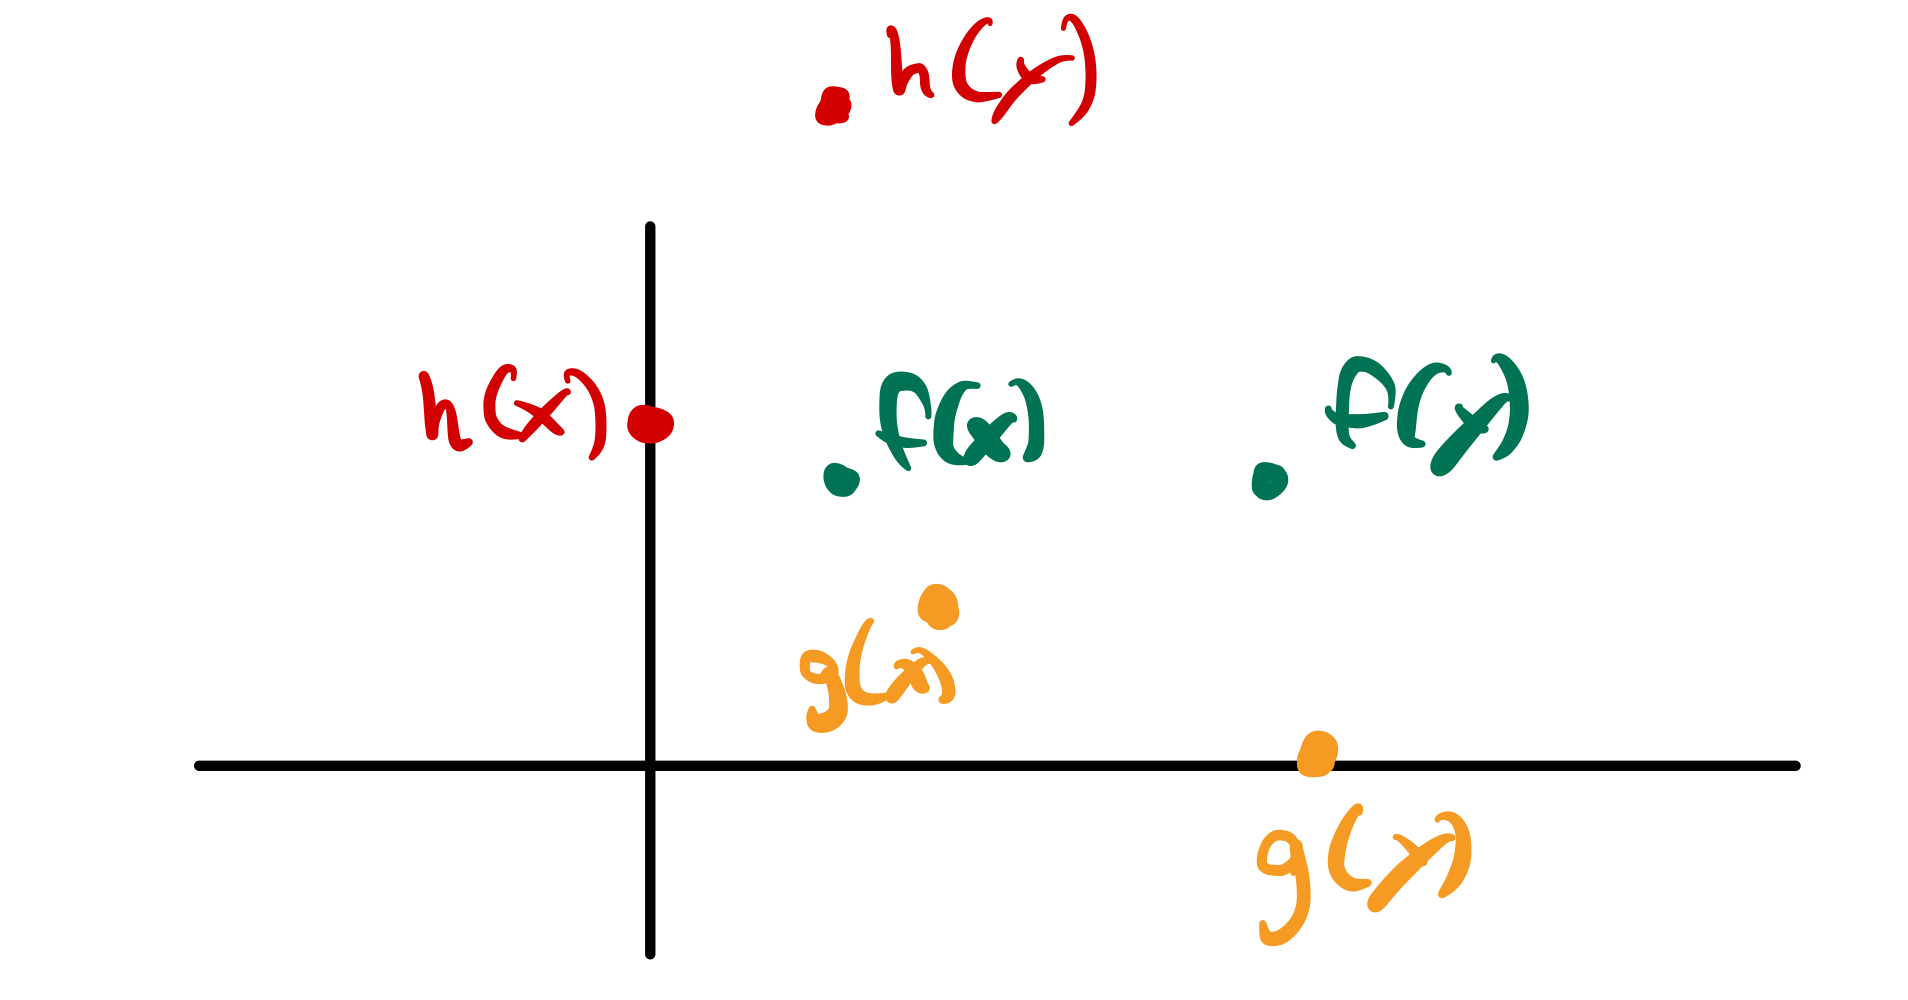
\includegraphics[scale=0.07]{complex.jpeg}
		\end{center}
		\vspace{-3mm}
		\caption*{The rotation trick to separate points}
		\end{figure}	

	Therefore, from the above, $\bar{C}_{\mathcal R} = \bar{C}_{\mathcal I} = C_b(E,\mathbb{R})$. Since $C_b(E, \mathbb{C}) = C_b(E,\mathbb{R}) + i \cdot C_b(E,\mathbb{R})$ we find that $C = C_{\mathcal{R}} + i \cdot C_{\mathcal{I}}$ is dense in $C_b(E, \mathbb{C})$.
\end{proof}
What is the magic of Stone-Weierstra\ss? Proving that families of functions are dense in other families is typically hard, a purely analytic $\varepsilon$-$N$ story. Stone-Weierstra\ss{} allows us to prove the density in a completely different way, only checking very simple algebraic properties! If we think about polynomials or exponential functions the algebraic properties are easily checked.\smallskip
\marginpar{\textcolor{red}{Lecture 15}}

The situation becomes even simpler if integrals are involved as linearity of integrals fits nicely to the properties of algebras.
\begin{llemma}
\begin{corollary}\label{cor_514}
	Let $(E,d)$ be a compact metric space and $C \subseteq C_b(E,K)$ a family that separates points, is closed under multiplication and contains $1$ (constant $1$ function). Then $C$ is separating for $\cM_1(E)$.
\end{corollary}
\end{llemma}
The examples that will appear in the sequal are typically polynomials or exponential functions on compact subsets of $\R$.
\begin{proof}[Proof]
	We start with a little trick on separating functions and algebras that relies on the linearity of integrals. Let $\mu,\: \nu \in \cM_1(E)$ with $\int_E g \dint \mu = \int_E g \dint \mu$ for all $g \in C$. Taking all linear combinations of functions in $C$ and calling them $C'$ then by linearity of integrals the equality also holds for all functions in $C'$ and $C'$ is an algebra of functions. Using the Stone-Weierstra\ss{} theorem, the equality of integrals holds for a dense subset of $C_b(E)$.
	\smallskip
	
	Fix $\varepsilon>0$. Then for all $f \in C_b(E)$ there exists $g \in C^{\prime}$ with $\left\Vert f - g \right\Vert_{\infty} < \varepsilon$ so that 
	\begin{align*}
		&\quad\Big| \int_E f \dint  \mu - \int_E f \dint \nu \Big|  \\ 
		&\leq \Big| \int_E f \dint \mu - \int_E g \dint \nu \Big| + \Big| \int_E g \dint \nu - \int_E g \dint \mu \Big| + \Big| \int_E g \dint \mu - \int_E f \dint \nu \Big| \\
		&\leq \left\Vert f - g \right\Vert_{\infty} \cdot \mu(E) + 0 + \left\Vert f - g \right\Vert_{\infty} \cdot \nu(E) = 2 \varepsilon.
	\end{align*}
	Since this works for all $\varepsilon > 0$ it follows that $$\int_E f \dint \mu = \int_E f \dint \nu,\quad \forall f\in C_b(E).$$ Recalling from Proposition \ref{theorem_4124} that $C_b(E)$ is separating for $\cM_1(E)$ we proved $\mu = \nu$. Hence, $C$ is separating for $\cM_1(E)$.
\end{proof}

\begin{lsuperwichtigersatz}
\begin{theorem}\label{coruniq}
	\begin{enumerate}[label=(\roman*)]
		\item Every measures $\mu\in \mathcal M_1([a,b])$ is uniquely determined by all integrals $$\int_{[a,b]} x^m \dint \mu(x),\quad m\in\N_0.$$
		\item The law of a \underline{bounded} real-valued random variable is determined by all it's moments, i.e. if $\E[X^m]=\E[Y^m]$ for all $m\in\N$, then $X\sim Y$.

	\end{enumerate}
\end{theorem}
\end{lsuperwichtigersatz}
\begin{proof}[Proof] All we need to do is to apply Corollary \ref{cor_514}.\smallskip

First note that $([a,b],|\cdot|)$ is a compact metric space. Define $C$ to be the family of monomials on $[a,b]$, that is $C = \{ x^m \colon m \in \mathbb{N}_0 \}$. Then $C$ is closed under multiplication, separates points in $[a,b]$ and contains the constant $1$ function. Hence, $C$ is a separating family for $\cM_1([a,b])$. But then, recalling the definition of a separating family,
\begin{align*}
	\int_{[a,b]} x^m \dint \mu(x)=\int_{[a,b]} x^m \dint \nu(x),\quad \forall m\in\N_0,
\end{align*}
implies $\nu=\mu$.\smallskip

The second claim follows from the first claim applied to the laws $\P_X$.
\end{proof}





\begin{lsuperwichtigersatz}
\begin{theorem}\label{cor_distributions_1}
	\begin{enumerate}[label=(\roman*)]
		\item Every measures $\mu \in \mathcal M_1([0,\infty)])$ is uniquely determined by all integrals $$\int_{[0,\infty)} e^{-\lambda x}\dint \mu(x),\quad \lambda>0.$$
		\item The law of a \underline{\smash{non-negative}} random variable is determined by it's Laplace transformation $L_X(\lambda) \coloneqq \E \big[ e^{- \lambda X} \big]$, $\lambda \geq 0$, i.e. if $L_X=L_Y$ then $X\sim Y$.
	\end{enumerate}
\end{theorem}
\end{lsuperwichtigersatz}
Of course part (ii) of the theorem also holds for non-positive random variables replacing the Laplace transformation by the moment generating function $M_X(t)=\E[e^{tX}]$ for all $t>0$.
\begin{proof}[Proof]
As in the previous proof we would like to apply Corollary \ref{cor_514} to the family of exponential functions, but there is a problem as $[0,\infty)$ is not compact. We apply a trick from Functional Analysis and use $E = [0, \infty]$ instead (the so-called one-point compactification).
\begin{luebung}
	$([0,\infty],d)$ is a compact metric space with $d(x,y):=|e^{-x}-e^{-y}|$. The metric is compatible with the usual convergence in $[0,\infty]$.
\end{luebung}
Note that convergence towards $\infty$ is divergence from basic analysis. Continuity of functions $f:[0,\infty]\to \R$ is best understood through sequences, $\lim_{n\to\infty} f(x_n)=f(x)$ and this takes in particular sequences that diverge to $\infty$. Hence, we can extend continuous functions on $[0,\infty)$ to continuous functions on $[0,\infty]$ if and only if $\lim_{x\to\infty} f(x)$ exists and in that case we must set $f(\infty)=\lim_{x\to\infty} f(x)$. For the exponential functions we thus define
\begin{align*}
	f_{\lambda}(x) \coloneqq \begin{cases}
			e^{- \lambda x} &: x>0 \\
			0 &: x = \infty, \lambda>0\\
			1 &: x = \infty, \lambda=0
			 \end{cases}.
\end{align*}
Then $C\coloneqq \{ f_{\lambda} \colon \lambda > 0 \}\subseteq C_b([0,\infty])$ separates points, $f_0 \equiv 1\in C$, and $f_{\mu}\cdot f_{\lambda} = f_{\mu + \lambda}$. Hence, $C$ separates probability measures on $\cB([0,\infty])$ and in particular measures on $\cB([0,\infty))$ which can be extended to $\cB([0,\infty])$ by extending a measure $\mu$ with $\bar{\mu}(\{ +\infty \} ) = 0$. That is, for $\nu, \mu\in \cM([0,\infty])$,
\begin{align*}
	&\quad \int_{[0,\infty)} e^{-\lambda x}\dint \mu(x)
	=\int_{[0,\infty)} e^{-\lambda x}\dint \nu(x),\quad \forall \lambda \geq 0\\
	& \Rightarrow \quad \int_{[0,\infty]}f \dint \bar \mu=\int_{[0,\infty]}f \dint \bar \nu,\quad \forall f\in C\\
	& \Rightarrow\quad \bar \mu=\bar \nu\\
	& \Rightarrow\quad \mu=\nu.
\end{align*}	
The second claim follows from the first claim applied to the laws $\P_X$.
	%	Let us assume $X$ and $Y$ take values in $[0,1]$, otherwise both are multiplied by the same constant which equally changes the moments. Now define $C$ to be the family of monomials, that is $C = \{ f_n \colon n \in \mathbb{N}_0 \}$ where $f_n=x^n$. Then $C$ is closed under multiplication, separates points in $[0,1]$ and contains the constant $1$ function. Hence, $C$ is a separating family for $\cM_1([0,1])$. But then, recalling the definition of a separating family,
%	\begin{align*}
%		\int_{[0,1]} f_n \dint \P_X= \E[X^n]  = \E[Y^n]= \int_{[0,1]} f_n \dint \mathbb{P}_Y,\quad \forall n \in \mathbb{N},
%	\end{align*}
%	implies $\mathbb{P}_X = \mathbb{P}_Y$, which is $X \sim Y$.
\end{proof}
Could we extend the same argument also to all measures on $\R$ (i.e. all random variables)? No! To do so we needed a family that is closed under multiplication (that leads to polynomials or exponentials) that converge at $+\infty$ and $-\infty$. Trying to find such a family is a good exercise to better understand the previous proofs. The trick that we get to know below is to replace the exponential functions by complex exponential functions.\smallskip

\begin{luebung}
	A little induction shows that all moments of $U\sim \mathcal U([a,b])$ are given by 
	\begin{align}\label{momuniform}
		\E[U^n]=\frac{1}{n+1}\sum_{k=0}^na^kb^{n-k}=\frac{b^{n+1}-a^{n+1}}{(n+1)(b-a)}	
	\end{align}
\end{luebung}
If for some reason one can show that a random variable has the moments from \eqref{B55}, then the random variable must be uniform. \smallskip

It is important to have an example in mind that shows that all moments do not uniquely determine the law of unbounded random variables. Here is nice counterexample that appears in the Black-Scholes theory of time-continuous financial markets. A random variable $X$ is called \textbf{log-normal} distributed if $X = \exp(Z)$, with $Z \sim \cN(0,1)$. Using substitution in $\P(X\leq t)=\P(Z\leq \log(t))=\int_{-\infty}^{\log(t)} \frac{1}{\sqrt{2\pi}} e^{-\frac{x^2}{2}}\dint x$ shows that $X$ has density $$ f_X(x) = \frac{1}{\sqrt{2 \pi}} \frac{1}{x} e^{- \frac{1}{2} \log(x)^2}\mathbf 1_{[0,\infty)}(x),\quad x\in\R.$$ From the moment generating function of the standard Gaussian distribution (see \ref{momg}) we obtain a formula for the moments: $\mathbf E\big[X^n \big] = \mathbf E \big[ e^{n\cdot Z} \big] = e^{\frac{1}{2}n^2}$. Next, we will write down an entire family of density functions that give the same moments but are log-normal densities. For $\alpha \in [-1,1]$ define
\begin{align*}
	f_{\alpha}(x) \coloneqq f_X(x) \cdot \big( 1 + \alpha \cdot \sin(2 \pi \log(x) \big)\mathbf 1_{[0,\infty)}(x),\quad x\in\R.
\end{align*}
Those functions are clearly non-negative and the computation below for $n=0$ shows they integrate to $1$, hence, they are densities. To prove the moments are identical to those of the log-normal distribution it suffices to show that 
\begin{align*}
	m(n) := \int_0^{\infty} x^n \cdot f_X(x) \cdot \sin(2 \pi \log(x)) \dint x = 0,\quad \forall n \in \mathbb{N}_0,
\end{align*}
and combine with $\int_\R x^n\cdot f_X(x)\dint x=\E[X^n]=e^{\frac{1}{2}n^2}$. Here is the computation:
\begin{align*}
	m(n) &= \int_{-\infty}^{\infty} e^{y\cdot n} \cdot f_X( e^y) \cdot \sin(2 \pi y ) \cdot e^y \dint y \\
		\overset{\text{subst. }y=z+n}&{=} \int_{-\infty}^{\infty} e^{zn + n^2} f_X(e^{z+n}) \sin(2 \pi z + 2 \pi n) e^{z+n} \dint z \\
		&= \frac{1}{\sqrt{2\pi}} e^{n^2} \int_{-\infty}^{\infty} e^{-\frac{1}{2}z^2-\frac{1}{2}n^2} \sin(2 \pi z) \dint z \\
		&= \frac{1}{\sqrt{2 \pi}} e^{\frac{1}{2}n^2} \underbrace{\int_{-\infty}^{\infty} e^{-\frac{1}{2}z^2} \sin(2 \pi z ) \dint z}_{ = 0 \text{, odd function and integrable}}=0.
\end{align*}
That's it.\smallskip

No doubt, the most exciting random variables (such as the Gaussian) are neither concentrated on a bounded interval nor are positive (or negative). In general the law is not determined only by moments as $\R$ (or $\R^d$) cannot be compactified such that enough functions are continuous on the compactification. Hence, an approach different from the Stone-Weierstra\ss{} theory is needed.\smallskip

The alternative approach uses the periodic structure of $e^{it}$:
\begin{ldef}
\begin{deff}

			For $\mu \in \cM_1(\mathbb{R}^d)$ the function $\varphi_\mu:\R^d\to\C$ defined by $$\varphi_{\mu}(t) \coloneqq \int_{\mathbb{R}^d} e^{\langle t,x \rangle} \dint\mu (x) \quad t\in \mathbb{R}^d,$$ is called the \textbf{characteristic function} (or Fourier transform) of $\mu$.
\end{deff}
\end{ldef}
The wording Fourier transformation comes from Fourier Analysis where integrable functions are studied through their Fourier transform $\hat{f}(x) \coloneqq \int e^{i\langle x, y \rangle} f(y) \dint y$. In probability theory people prefer to use the name characteristic function as a random variable is uniquely characterised through the characteristic functions.\smallskip

As always we can either define objects for probability measures or random variables with the corresponding law. Since the characteristic function is such an important object let us fix the other notation as well:
\begin{ldef}
\begin{deff}
			For a random vector $X$ the function $\varphi_X:\R^d\to\C$ defined by $$\varphi_X(t) \coloneqq \E[e^{i \langle t, X \rangle}] = \varphi_{\mathbb{P}_X}(t), \quad t\in \mathbb{R}^d,$$ is called the textbf{characteristic function of $X$}.
\end{deff}
\end{ldef}
			 The characteristic function plays exactly the same role as moment generating function $\mathcal M_X$, or the distribution function $F_X$. It is just a function with certain properties (see below) that can be used to study more complicated mathematical objects such as measures or random variables. The major advantage of the characteristic function is that $\varphi$ is always well-defined because $\varphi_X$ is always defined as $\lvert e^{ix} \rvert = 1$.\smallskip

Here are some properties that indicate that characteristic functions are useful to work with:
\begin{llemma}
\begin{lemma}\label{lemma_5111}
	Let $X$ be a random vector and $\varphi_X \colon \mathbb{R}^d \to \mathbb{C}$ the characteristic function.
	\begin{enumerate}[label=(\roman*)]
		\item $\varphi_X(0) = 1$ and $\lvert \varphi_X(t) \rvert \leq 1$ for all $t \in \mathbb{R}^d$.
		\item $\varphi_{aX+b}(t) = \varphi_X(a t)  e^{i\langle b,t \rangle}$ for all $ a \in \mathbb{R}$ and $b\in \mathbb{R}^d$.
		\item $\varphi$ is real-valued if and only if $X$ is symmetric, i.e. $\mathbb{P}_X = \mathbb{P}_{-X}$.
		\item $\varphi_{X+Y} = \varphi_X \cdot \varphi_Y$ if $X$ and $Y$ are independent.
	\end{enumerate}
\end{lemma}
\end{llemma}
\begin{proof}[Proof]
	If you are not used to integrals for complex-valued functions the arguments are a bit more complicated than one might think.
	\begin{luebung}
		To get started please check the linearity $\int (\alpha f+\beta g)\dint \mu=\alpha \int f \dint \mu+\beta \int f \dint \mu$ for $\alpha, \beta \in\C$ of complex integrals by using the definition and properties of real integrals.
	\end{luebung}
	\begin{enumerate}[label=(\roman*)]
		\item Let us first assume the usual triangle inequality also for complex integrals. Then we obtain
			\begin{align*}
				\lvert \varphi_X(t) \rvert 
				= \big| \E \big[ e^{i \langle t,X \rangle} \big] \big| 
				= \Big| \int_{\Omega} e^{i \langle t, X(\omega) \rangle} \dint \mathbb{P}(\omega) \Big|
				\overset{\Delta}{\leq} \int_{\Omega} \big| e^{i \langle t, X(\omega) \rangle} \big| \dint \mathbb{P}(\omega)
				= \int_\Omega 1\dint \P(\omega) = 1.
			\end{align*}
			The triangle inequality $|\int_\Omega f\dint \mu|\leq \int_\Omega |f|\dint \mu$ is more complicated than one might think. Suppose $\varphi$ is the angle from the polar coordinate representation of $\int_\Omega f\dint \mu$. Then
			\begin{align*}
				\Big|\int_\Omega f \dint \mu \Big| = e^{-i\varphi} \int_\Omega f \dint \mu
				=\int_\Omega e^{-i\varphi} f \dint \mu
				=\int_\Omega \mathcal{R}e(e^{-i\varphi} f) \dint \mu
				\leq \int_\Omega |e^{-i\varphi} f| \dint \mu
				= \int_\Omega  |f| \dint \mu.
			\end{align*}
			The first equality holds as multiplying with $e^{-i\varphi}$ is a rotation, the second is linearity, the third holds as $|\cdot|\in \R$ so that the imaginary part of the integral vanishes, and the fourth is monotonicity for real-valued integrals. Finally, the fifth equality is $|e^{-i\varphi}f|=|e^{-i\varphi}||f|=|f|$.
		\item
			Write it down yourself!
		\item Recall that
			$e^{-i\theta} = \cos(-\theta) + i \sin(-\theta) = \cos(\theta) - i \sin(\theta) = \overline{e^{i \theta}}$, hence, 
			\begin{align*}
				\varphi_{-X}(t) = \E \big[ e^{-i \langle X, t \rangle} \big] = \E \big[ \overline{ e^{i \langle X, t \rangle}} \big] = \overline{\E [ e^{i \langle X, t \rangle}]} = \overline{\varphi_X(t)},
			\end{align*}
			where we used
			\begin{align*}
				\overline{\int f\dint \mu}=\overline{\int \mathcal{R}e(f)\dint \mu+i\int \mathcal{I}m(f)\dint \mu}=\int \mathcal{R}e(f)\dint \mu-i\int \mathcal{I}m(f)\dint \mu=\int \overline{f}\dint \mu.
			\end{align*}
			The claim now follows immediately.
			\item The proof is essentially the same that we have seen for moment generating functions in Proposition \ref{P7}. All we need to do is to extend Theorem \ref{un} to complex-valued functions. But this is simple using the linearity from above:
			\begin{luebung}
				Check that $\E[f(X)g(Y)]=\E[f(X)]\E[g(Y)]$ holds for independent random variables $X$ and $Y$.
			\end{luebung}
		%\begin{align*}
		%	\E[f(X)f(Y)]&=\E[\mathcal{R}e (f)(X)\mathcal{R}e (g)(X)]+i\E[\mathcal{R}e (f)(X)\mathcal{I}m (g)(X)]\\
		%	&\quad +i\E[\mathcal{I}m (f)(X)\mathcal{R}e (g)(X)]-\E[\mathcal{I}m (f)(X)\mathcal{I}m (g)(X)]\\
		%\overset{\ref{un}}&{=}\E[\mathcal{R}e (f)(X)]\E[\mathcal{R}e (g)(X)]+i\E[\mathcal{R}e (f)(X)]\E[\mathcal{I}m (g)(X)]\\
		%	&\quad +i\E[\mathcal{I}m (f)(X)]\E[\mathcal{R}e (g)(X)]-\E[\mathcal{I}m (f)(X)]\E[\mathcal{I}m (g)(X)]\\
		%	&=(\E[\mathcal{R}e (f)(X)]+\E[\mathcal{I}m (f)(X)])\cdot (\E[\mathcal{R}e (g)(X)]+\E[\mathcal{I}m (g)(X)])\\
		%	&=\E[f(X)]\cdot \E[g(Y)].
		%\end{align*}
		But then 
		\begin{align*}
			\varphi_{X+Y}(t)=\E[e^{i\langle t,X+Y\rangle}]=\E[e^{i\langle t,X\rangle}]\cdot \E[e^{i\langle t,Y\rangle}]=\varphi_X(t)\cdot \varphi_Y(t),
		\end{align*}
		for all $t\in\R$.
	\end{enumerate}
\end{proof}
	\marginpar{\textcolor{red}{Lecture 16}}

	To get a feeling let us check some examples.
	\begin{example}
		Using the discrete computation rule from \eqref{expec} yields
		$$\varphi_{\text{Poi}(\lambda)}(t) = \E \big[ e^{itX} \big] = \sum_{k=0}^{\infty} e^{-\lambda} e^{itk} \frac{\lambda^k}{k!} = e^{\lambda (e^{it}-1)}e^{\lambda ( e^{it} - 1)},\quad t\in\R,$$
		and
		\begin{align*}
			\varphi_{\text{Bin}(n,p)}(t)
			&=\E\big[ e^{itX} \big]\\
			&= \sum\limits_{k=0}^{n} {n\choose k} e^{itk}p^k (1-p)^{n-k}\\
			&= \sum\limits_{k=0}^{n}{n\choose k} (p  e^{it})^k (1-p)^{n-k} = \big( 1 - p +p  e^{it} \big)^n,\quad t\in\R.
		\end{align*}
		The second example can also be computed from (iv) of Lemma \ref{lemma_5111} using
		\begin{align*}
			\varphi_{\text{Ber}(p)}(t)=\E[e^{itX}]=e^{it}p+(1-p)e^{it0},\quad t\in\R,
		\end{align*}
and that a binomial random variable is a sum of $n$ independent Bernoulli random variables.

		
		%$$\varphi_{\text{Bin}(n,p)}(t) = \big( 1- p+ p \cdot e^{it} \big)^n$$
		%Why? $\mathbf E \big[ e^{itX} \big] = \sum\limits_{k=0}^{n} {n\choose k} e^{itk}p^k (1-p)^{n-k} = \sum\limits_{k=0}^{n} (p \cdot e^{it})^k (1-p)^{n-k} = \big( 1 - p +p \cdot e^{it} \big)^n$
	\end{example}
	
		\begin{example}
			Using the computation rule from \eqref{expec} yields
			$$\varphi_{\mathcal U([0,a])}(t) = \frac{e^{iat}-1}{iat},\quad t\in\R.$$
			The computation is straight forward using the definition of the complex integral:
			\begin{align*}
				\E \big[ e^{itX} \big] 
				&= \int_0^a e^{itx} \frac{1}{a} \dint x\\
				  &= \frac{1}{a} \int_0^a \cos(t  x) \dint x + \frac{1}{a} i \int_0^a \sin(t  x) \dint x \\
					&= \frac{1}{at} \big( [ \sin(tx)]_0^a - i [\cos(tx) ]_0^a \big) \\
					&= \frac{1}{at} \big( \sin(at) - i \cos(ax) + i \big)   \\
					\overset{i^2=-1}&{=} \frac{1}{at} \frac{1}{i} \big( \cos(at) + i \sin(at) + i^2 \big) 
					= \frac{e^{iat}-1}{a i  t}
			\end{align*}
		\end{example}
	Unfortunately, it is not always the case that the complex integrals can be computed that easily. In many instances countour integrals $\int_\gamma f(z)\dint z$ need to used in order to compute $\int_\R f(x)\dint x$. If you know about contour integration this is a good exercise, otherwise it is a good reason to learn about contour integration!
	\begin{luebung}
			\begin{example}
		$$\varphi_{\cN(\mu,\sigma^2)}(t) = e^{i \mu t}e^{-\frac{\sigma^2}{2}t^2},\quad t\in\R,$$
		and 
		$$\varphi_{\text{Exp}(\lambda)}(t) = \frac{\lambda}{\lambda - i  t},\quad t\in\R.$$
		\end{example}
	\end{luebung}
Apart from being nice to compute with there must be a deeper reason to study characteristic functions. The fundamental theorem on characteristic functions states that the complex exponential functions are separating for $\cM_1(\R^d)$ or, formulated in the langueage of random variables, the law of a random variable is uniquely determined by the characteristic function. Indeed, this is the justification for the name, the law is characterised by the characteristic function.
\begin{lsuperwichtigersatz}
\begin{theorem}\label{CF}
	\begin{enumerate}[label=(\roman*)]
		\item Every measures $\mu \in \mathcal M_1(\R^d)$ is uniquely determined by all integrals $$\int_{\R^d} e^{i \langle t,x\rangle}\dint \mu(x),\quad t\in\R^d.$$
		\item The law of a random vector $X$ is determined by it's characteristic function, i.e. if $\varphi_X=\varphi_Y$ then $X\sim Y$.
	\end{enumerate}\end{theorem}
\end{lsuperwichtigersatz}
\begin{proof}[Proof]
	Since $C_c(\R^d)$ is separating by Proposition \ref{theorem_4124} it suffices to prove that the complex exponentials are dense in $C_c(\R^d)$, then we can proceed similarly (but with an extra trick) to the proof of Corollary \ref{cor_514}. The main idea of the proof is best understood in pictures. Let us fix two measures $\mu_1, \mu_2\in \cM_1(\R^d)$, $f\in C_c(\R^d)$ and suppose $f$ that vanishes outside of a box $[-\frac{k}{2}, \frac{k}{2} ]^d$. 
	\begin{figure}[h]
		\vspace{-3mm}
		\begin{center}
			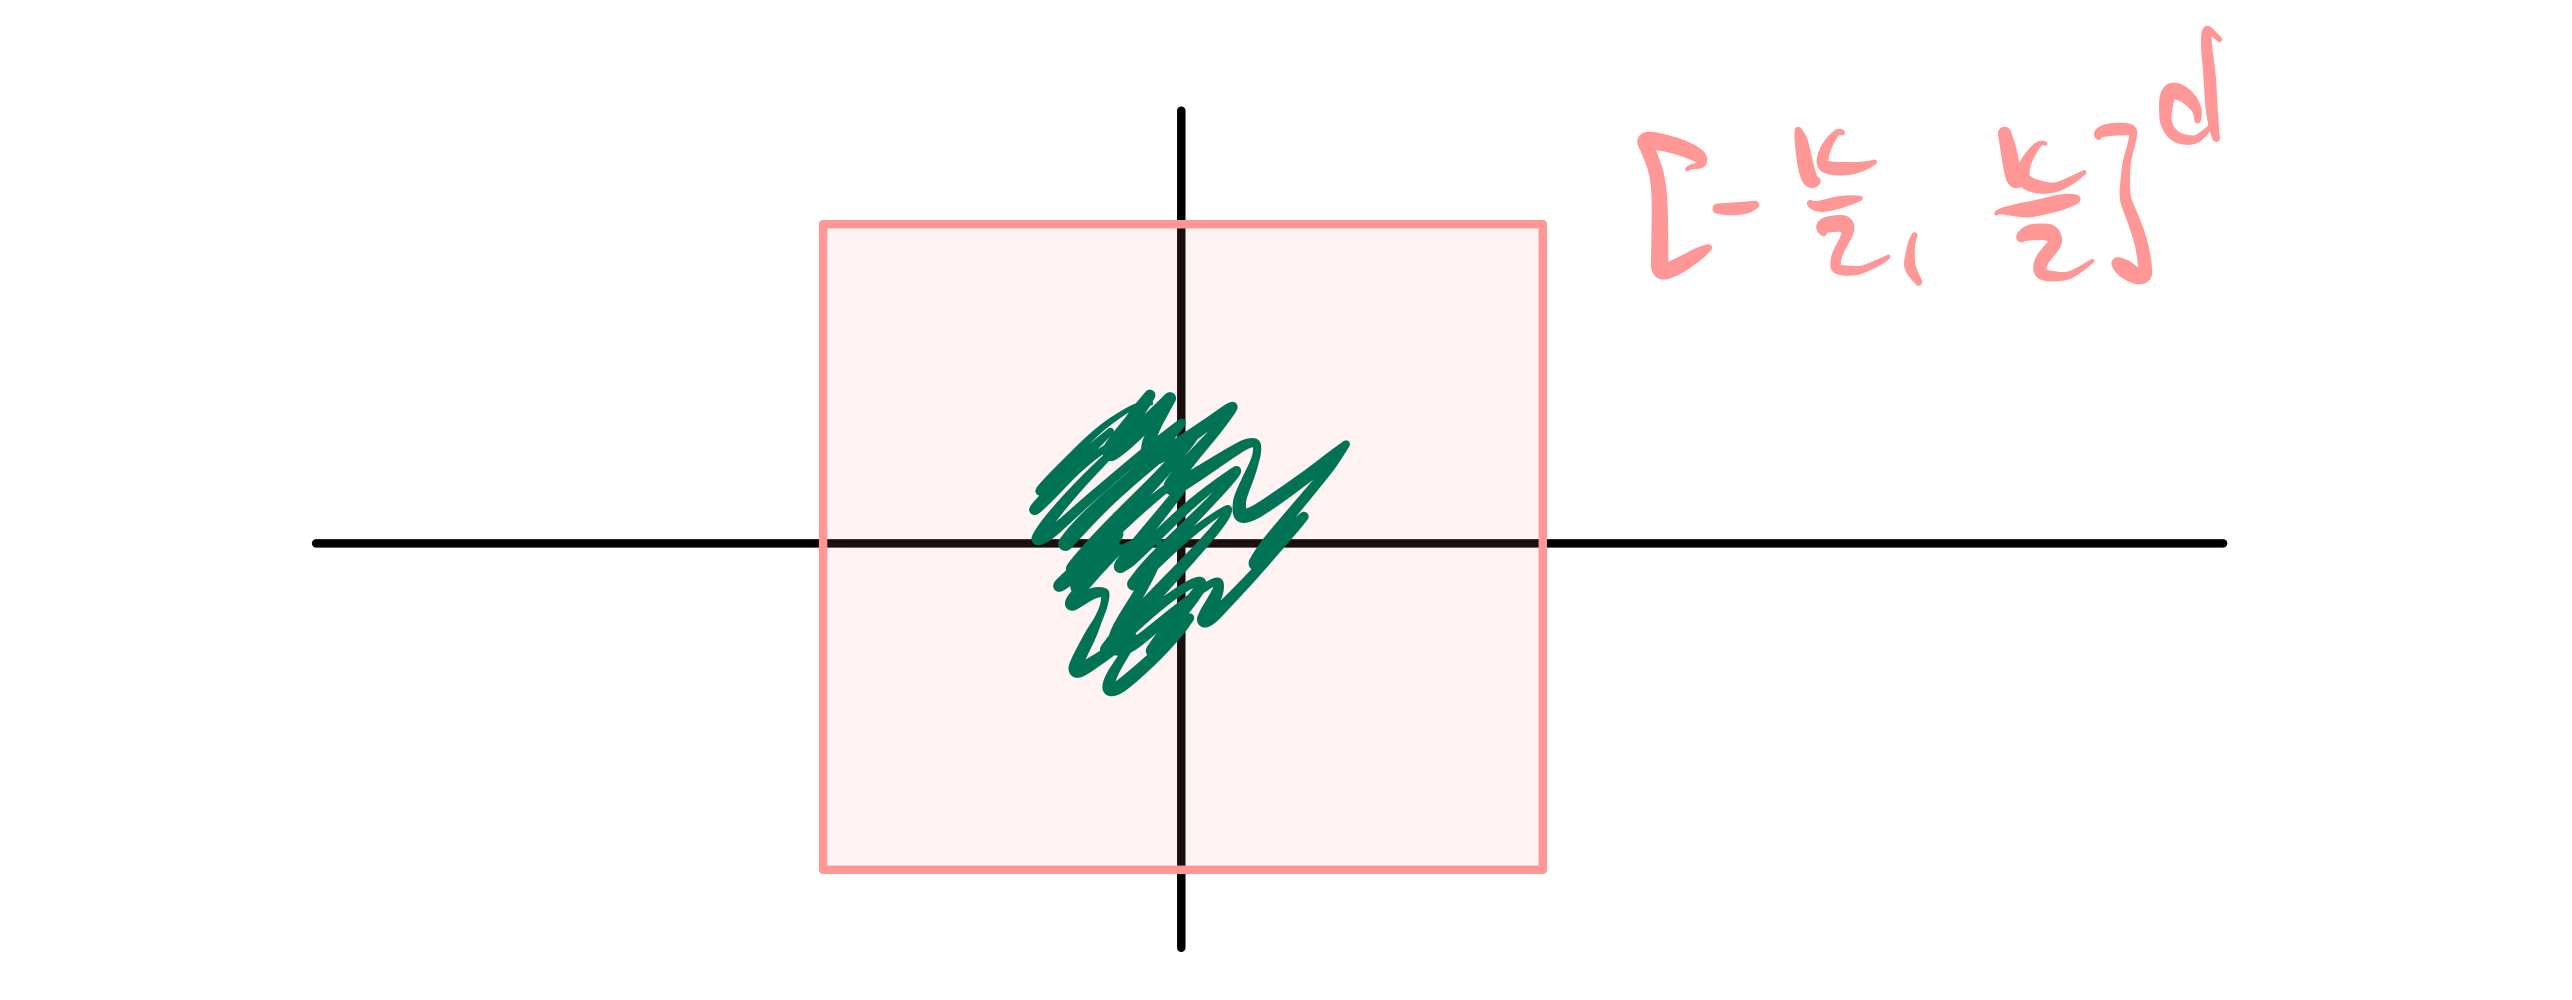
\includegraphics[scale=0.07]{compact.jpeg}
		\end{center}
		\vspace{-3mm}
		\caption*{The support of $f$}
		\end{figure}
	By enlarging $k$ we can choose $k$ such that $\mu_i \big( \mathbb{R}^d  \setminus (k,k)^d \big) < \varepsilon$ for a fixed $\varepsilon >0$ (continuity of measures or Proposition \ref{prop_4120}). Next we define
	\begin{align*}
		g_m \colon \mathbb{R}^d \to \mathbb{C},\quad g_m (x) = e^{ i \langle \frac{\pi m}{k}, x \rangle },\quad m \in x,\mathbb{Z}^d,
	\end{align*}
	and $C_k$ as the algebra of finite linear combinations of the $g_m$. Here is the important point of the functions $g_m$, they are periodic. For $n \in \mathbb{Z}^d$ they satisfy
			\begin{align*}
				g_m(x+2 k n) = e^{ i \langle \frac{\pi m}{k}, x \rangle } \cdot \underbrace{e^{ i \langle \frac{\pi m}{k}, 2k n \rangle }}_{=1} = g_m(x),
			\end{align*}
			as $e^{2\pi l}=1$ for all $l\in\Z$.	Hence, the entire family $C_k$ is periodic!
			\begin{figure}[h]
				\vspace{-1mm}
				\begin{center}
					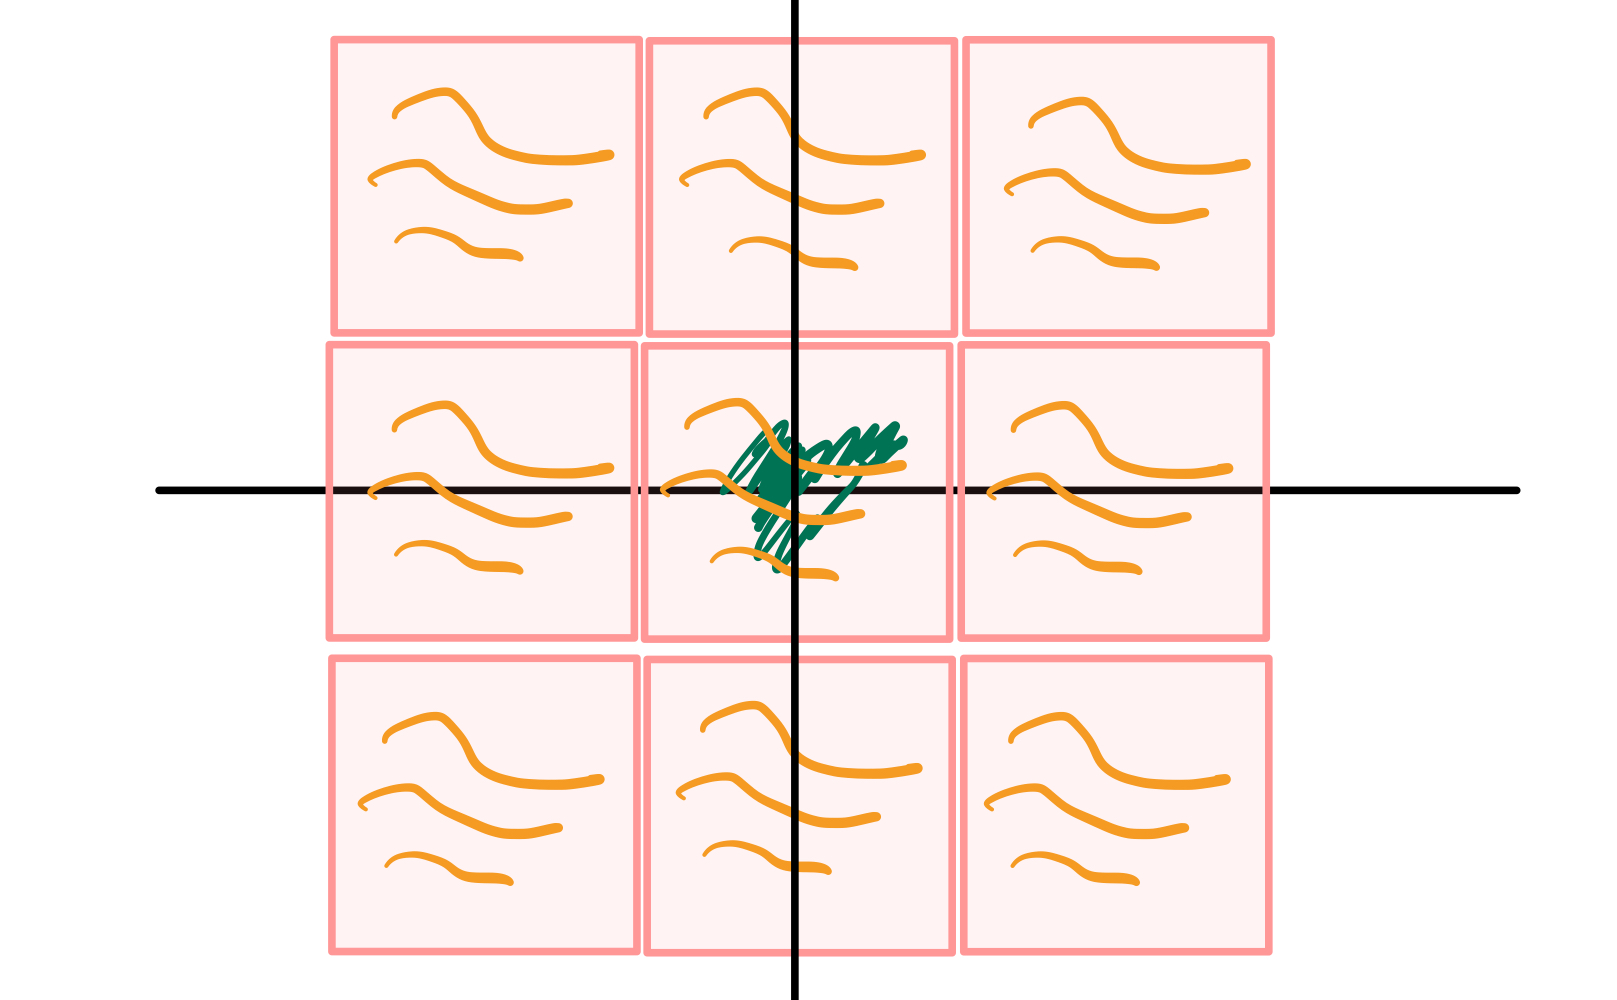
\includegraphics[scale=0.07]{periodic.jpeg}
				\end{center}
				\vspace{-3mm}
				\caption*{Periodic function $g\in C_k$}
				\end{figure}			

			This is important to us as bounding $g\in C_k$ on $[-k,k]^d$ will automatically bound $g$ everywhere. Restricting $C_k$ to $[-k,k]^d$ the class is separating (this needs the $1 /k$ in the scalar product as without it the functions would be periodic for a smaller box taking the same values on shifts of the smaller boxes in the larger box). The Stone-Weierstra\ss{} approximation theorem now implies that there is $g \in C_k$ with 
			\begin{align*}
				\sup_{x\in [-k,k]^d}\lvert f(x) - g(x) \rvert < \varepsilon.
			\end{align*}
			Since $g$ is close to $f$ on $[-k,k]^d$ we can also use the periodicity to bound $g$ on $\R^d$:
			\begin{align*}
				\sup_{x\in\R^d}|g(x)|=\sup_{x\in [-k,k]^d} \lvert g(x) \rvert &\leq \sup_{x\in [-k,k]^d}\lvert f(x) - g(x) \rvert + \sup_{x\in [-k,k]^d} \lvert f(x) \rvert 
					\leq \varepsilon + \left\Vert f \right\Vert_{\infty}.
			\end{align*}
			Putting everything together, the above thoughts yields (please compare the proof of Corollar \ref{cor_514})
			\begin{align*}
				&\quad\Big\lvert \int_{\mathbb{R}^d} f \dint \mu_1 - \int_{\mathbb{R}^d} f \dint \mu_2 \Big\rvert \\
				&\leq \Big\lvert \int_{\mathbb{R}^d} f \dint \mu_1 - \int_{\mathbb{R}^d} g \dint \mu_1 \Big\rvert + \underbrace{ \Big\lvert \int_{\mathbb{R}^d} g \dint \mu_1 - \int_{\mathbb{R}^d} g \dint \mu_2 \Big\rvert }_{= 0 \text{ by assumption}} + \Big\lvert \int_{\mathbb{R}^d} g \dint \mu_2 - \int_{\mathbb{R}^d} f \dint \mu_2 \Big\rvert  \\
&\leq \int_{[k,k]^d}|f-g|\dint \mu_1+ \int_{([k,k]^d)^c}|f-g|\dint \mu_1+ \int_{[k,k]^d}|f-g|\dint \mu_2+ \int_{([k,k]^d)^c}|f-g|\dint \mu_2\\
				& \leq \mu_1 \big( [-k,k]^d \big) \cdot \varepsilon + \mu_1 \big( ([-k,k]^d)^c \big) \cdot ( \varepsilon + \left\Vert f \right\Vert_{\infty}) 
				 +   \mu_2 \big( [-k,k]^d \big)
				+ \mu_2 \big( ([-k,k]^d)^c \big) \cdot ( \varepsilon + \left\Vert f \right\Vert_{\infty}) \\
				&\leq 2 \varepsilon + 2 \varepsilon \big( \varepsilon + \left\Vert f \right\Vert_{\infty} \big).
			\end{align*}
			For the inequalities we used that $\mu_i$ are probability measures, $|f-g|\leq |f|+|g|$, and that $\mu_i$ only have mass at most $\varepsilon$ outside of the chosen box. Since $\varepsilon$ was arbitrary we proved $\int f \dint \mu_1 = \int f \dint \mu_2$.\smallskip

			The second claim follows from the first claim applied to the laws $\P_X$.
\end{proof}
Of course one might ask why one might be interested in computing moments (for bounded random variables) or Laplace transformations (for non-negative random variables) if there is one general theorem that states that characteristic functions uniqueley determine all real random variables. This is because it is easier to compute moments or Laplace transformations these are the preferred tools in the special situations when they are sufficiently powerful.\smallskip

\begin{lwarnhinweis}
So far we are used to describe random variables through their cummulative distribution function, density, or discrete probability weights. An alternative way is to describe random variables directly in terms of their chracteristic functions, which, according to the previous theorem, is as good as using the CDF.
\end{lwarnhinweis}
The drawback of using characteristic functions is that one needs to compute expectations (integrals) for complex functions. At the same time this is the big advantage, too, as complex integration has wonderful tricks to offer. \smallskip

In many examples the uniquneness is applied as follows. In order to identify the distribution of a random variable (such as a sum of other random variables) one tries to compute the characteristic function. If that characteristic function is already known we can identify the law. We already know this concept from Proposition \ref{P7} and the example below but always used the trick without a proof. Here is another little exercise to play with the examples, Lemma \ref{lemma_5111} and uniqueness theorem.
\begin{luebung}
	Check that 
	\begin{itemize}
		\item If $Y\sim \mathcal N(0,1)$, then $Y:=\sigma X+Y\sim \mathcal N(\mu,\sigma^2)$.
		\item
		If $X \sim \cN(\mu_1,\sigma_1^2)$ and $Y \sim \cN(\mu_2,\sigma_2^2)$ are independent, then $$X+Y \sim \cN(\mu_1+\mu_2, \sigma_1^2 + \sigma_2^2).$$
	\item
		If $X \sim \text{Poi}(\lambda)$ and $Y \sim \text{Poi}(\beta)$ are independent, then $X + Y \sim \text{Poi}(\lambda + \beta)$. 
	\end{itemize}
\end{luebung}



\section[Weak convergence on $\mathcal B(\R)$]{Weak convergence on $\mathcal B(\R^d)$}
We can finally return to the question of weak convergence. Recall from Propositon \ref{most_useful_characterization_weak_convergence} that a sequence of probability measures $(\mu_n)$ converges weakly to $\mu$ (equivalently a sequence of random variables $(X_n)$ converges in distribution to $X$) if and only if
\begin{enumerate}[label=(\roman*)]
	\item $\{\mu_n:n\in\N\}$ is tight,
	\item $ \lim_{n\to\infty} \int_E f \dint \mu_n = \int_E f \dint \mu$ for \underline{some} separating family $C \subseteq C_b(E)$ of $\cM_1(E)$.
\end{enumerate}
We have identified separating families in the previous section. It now remains to identify situations in which the tightness trivially holds (bounded and non-negative) and give a handable criterion to check the tightness (convergence of characteristic functions). We keep the order of the previous section and first deal with the simple cases:
\begin{lsatzwichtig}
\begin{theorem}
	\begin{enumerate}[label=(\roman*)]
		\item Suppose that $\mu,\mu_1,...\in \mathcal M_1([a,b])$, then 
	\begin{align*}
		\mu_n \overset{\text{(w)}}{\longrightarrow} \mu,\: n \to \infty \quad\Leftrightarrow \quad \lim_{n\to\infty}\int_{[a,b]} x^m\dint \mu_n(x)=\int_{[a,b]} x^m\dint \mu(x),\quad \forall m\in\N_0.
	\end{align*}
	\item Suppose that $X,X_1,...$ are random variables with values in $[a,b]$, then 
	\begin{align*}
		X_n \overset{\text{(d)}}{\longrightarrow} X,\: n \to \infty \quad\Leftrightarrow \quad \lim_{n\to\infty}\E[X_n^m]=\E[X^m], \quad \forall m\in\N_0.
	\end{align*}
\end{enumerate}
\end{theorem}
\end{lsatzwichtig}
\begin{proof}[Proof]
	(ii) follows from (i) by the definition of convergence in distribution with the measures $\mu_n:=\P_{X_n}$ using that $\E[X_n^m]=\int x^m \dint \P_{X_n}(x)$.\smallskip

	(i) The situation is simple as $([a,b],|\cdot|)$ is compact. Hence, every sequence of measures is automatically tight (choose $K=[a,b]$ in the definition of tightness). According to Proposition \ref{most_useful_characterization_weak_convergence} only convergence of integrals needs to be checked for a separating family. Since the family of monomials $C=\{x^m:m\in\N_0\}$ is separating according to Theorem \ref{coruniq} the proof is complete.
\end{proof}

The situation is very similar for non-negative (or non-positive) sequences of random variables. In contrast to bounded sequences we now need convergence of the exponential moments (Laplace transformation):
\begin{lsatzwichtig}
	\begin{theorem}
		\begin{enumerate}[label=(\roman*)]
			\item Suppose that $\mu,\mu_1,...\in \mathcal M_1([0,\infty))$, then 
		\begin{align*}
		\hspace{-4mm}	\mu_n \overset{\text{(w)}}{\longrightarrow} \mu,\: n \to \infty \quad\Leftrightarrow \quad \lim_{n\to\infty}\int_{[0,\infty)} e^{-\lambda x}\dint \mu_n(x)=\int_{[0,\infty)} e^{-\lambda x}\dint \mu(x),\,\, \forall \lambda >0.
		\end{align*}
		\item Suppose that $X,X_1,...$ are non-negative random variables, then 
		\begin{align*}
			X_n \overset{\text{(d)}}{\longrightarrow} X,\: n \to \infty \quad\Leftrightarrow \quad \lim_{n\to\infty} L_{X_n}(\lambda)=L_X(\lambda), \quad\forall \lambda>0.
		\end{align*}
	\end{enumerate}
	\end{theorem}
	\end{lsatzwichtig}
	\begin{proof}[Proof]
		(ii) follows from (i) by the definition of convergence in distribution with the measures $\mu_n:=\P_{X_n}$ using that $L_{X_n}(\lambda)=\int e^{-\lambda x} \dint \P_{X_n}(x)$.\smallskip
	
		(i) We argue as in the proof of Theorem \ref{cor_distributions_1}. Compactifying $[0,\infty]$ and extending the measures trivially to measures $\bar \mu_n$ yields a sequence of measures in a compact space. As in the previous proof the sequence is automatically tight (choose $K=[0,\infty]$). 
		According to Proposition \ref{most_useful_characterization_weak_convergence} only convergence of integrals needs to be checked for a separating family. Since the family of exponentials $C\coloneqq \{ f_{\lambda} \colon \lambda > 0 \}$ is separating according to Theorem \ref{cor_distributions_1} the proof is complete.
	\end{proof}
The most general theorem is L\'evy's continuity theorem. Without any further assumption weak convergences is equivalent to convergence of the characteristic functions. 
%Erst beschränkt und positiv. Dann R. Dann C.

%\textbf{Goal:}
%	\begin{align*}
%		X_n \overset{(d)}{\longrightarrow} X, \: n\to \infty \: &\Leftrightarrow \: F_{X_n} \longrightarrow F, \: n\to \infty, \text{ at points of continuity} \\
%		&\overset{?}{\Leftrightarrow} \varphi_{X_n} \longrightarrow \varphi_X, \: n \to \infty
%	\end{align*}
%	\begin{lemma1}
%		Let $\mu \in M_1( \mathbb{R}^d)$, then
%		\begin{align*}
%			\lvert \varphi_{\mu}(t) - \varphi_{\mu}(s) \lvert^2 \leq 2 \cdot \big( 1 - \mathcal{R}e( \varphi_{\mu}(t-s)) \big), \:\: \forall s,t 
%		\end{align*}
%	\end{lemma1}
%	\begin{proof}
%		$L^2(\Omega,\cA,\mathbb{P})$ is a Hilbertspace with $\langle f, g \rangle = \int f \cdot \bar{g} \dint \mu$ also if we consider $f \colon \Omega \to \mathbb{C}$ and the complex integral $\int f \dint \mu \coloneqq \int \cR e(f) \dint \mu + i \int Im(f) \dint \mu$.
%		\begin{align*}
%			\big\lvert \varphi_{\mu}(t) - \varphi_{\mu}(s) \big\rvert^2 &= \Big\lvert \int_{\mathbb{R}^d} \big( e^{i \langle t,x \rangle}- e^{i \langle s,x \rangle} \big) \dint \mu (x) \Big\rvert^2 \\
%			&= \Big\lvert \int_{\mathbb{R}^d} \big( e^{i \langle t,x \rangle} - 1 \big) e^{i \langle s, x \rangle} \dint \mu(x) \Big\rvert^2 \\
%			\overset{ \text{C-S}}&{\leq} \int_{\mathbb{R}^d} \lvert e^{ i \langle t-s,x \rangle} - 1 \rvert^2 \dint \mu(x) \cdot \underbrace{\int_{\mathbb{R}^d} \underbrace{\lvert e^{i \langle s,x \rangle} \rvert^2}_{=1} \dint \mu(x) }_{=1} \\
%			\overset{\lvert z \rvert^2 = z \cdot \overline{z}}&{=} \int_{\mathbb{R}^d} \big( e^{i \langle t - s, x \rangle} - 1\big) \cdot \big( e^{-i \langle t-s,x \rangle} - 1 \big) \dint \mu(x) \\
%			&= 2 \cdot \big(1 - \cR e(\varphi_{\mu}(t-s)) \big)
%		\end{align*}
%	\end{proof}
%	Recall: $f \colon E \to F$ is uniformly continuous if $\forall \varepsilon > 0 \exists \delta > 0 \colon \: d(x,y) <\delta \Rightarrow d \big( f(x),f(y) \big) < \varepsilon$. Now we take a family of continuous functions and wanr the choice of $\delta$ to be the same for all $f$ $\rightsquigarrow$ family $\cF$ is uniformly uniformly continuous.
%	\begin{deff1}
%		Let $(E,d)$ be a metric space. A family $(f_i)_{i\in I}$ of maps $f_i \colon E \to \mathbb{R}$ is called \underline{\smash{uniformly equicontinuous}} if
%		\begin{align*}
%			\forall \varepsilon > 0 \: \exists \delta > 0 \colon \: d(x,y) < \delta \: \Rightarrow \: \lvert f_i(x) - f_i(y) \rvert < \delta \:\: \forall i \in I
%		\end{align*}
%	\end{deff1}
%	\begin{theorem}
%		If $\cF \subseteq M_1( \mathbb{R}^d ) $ is tight, then $\{ \varphi_{\mu} \colon \mu \in \cF \}$ is uniformly equicontinuous. In particular, every characteristic function is uniformly continuous.
%	\end{theorem}
%	\begin{proof}
%		Recall $\big( M_1(\mathbb{R}^d), d_P \big)$ is indeed a metric space (even Polish). Fix $\varepsilon > 0$. Since $\cF$ is tight there is $N\in \mathbb{N}$ with $\mu \big( [ -N, N ]^d \big) > 1- \frac{\varepsilon^2}{6}$. Since $[-N,N]^d$ is compact there is a $\delta > 0$ such that $ \lvert 1 - e^{i \langle u,x \rangle} \rvert < \frac{\varepsilon^2}{6}$ for all $x \in [-N,N ]^d$ and all $\lvert u \rvert < \delta$ (Use continuity of $(u,x) \mapsto 1 - e^{i \langle u,x \rangle}$ and cover with finitely many balls, take the smallest corresponding $\delta$ which then works for all $x$ at onexe). Hence,
%		\begin{align*}
%			1 - \cR e  \big( \varphi_{\mu}(u) \big) &\leq \int \lvert 1 - e^{i \langle u,x \rangle} \rvert \dint \mu(x) \\
%			&\leq 2 \cdot \mu \big( ([-N,N]^d)^C \big) + \frac{\varepsilon^2}{6} \mu \big( [-N,N]^d \big)  \\
%			&\leq \frac{\varepsilon^2}{3} + \frac{\varepsilon^2}{6} = \frac{\varepsilon^2}{2}
%		\end{align*}
%		for all $\mu \in \cF$. Now we use the lemma to get the uniform bound needed for the definition of uniformly equicontinuity.
%	\end{proof}
%	\begin{prop1}[limits of uniformly uniformly seq. of functions are unif. cont.]
%		Let $(E,d)$ be a metric space, $f,f_1,f_2,...\colon E \to \mathbb{R}$ with $f_n \to f$ pointwise. If $(f_n)_{n\to\infty}$ is uniformly equicontinuous, then
%			\begin{enumerate}[label=(\roman*)]
%				\item $f$ is uniformly continuous
%				\item $f_n \to f$ uniformly on compacts, i.e. $\sup\limits_{x\in K} \lvert f_n(x) - f(x) \rvert \to 0$ for all $K \subseteq E$ compact.
%			\end{enumerate}
%	\end{prop1}
%	\begin{proof}
%		\begin{enumerate}[label=(\roman*)]
%			\item
%				Let $\varepsilon >0$ and fix $\delta >$ with $\lvert f_n(x) - f_n(y) \rvert < \varepsilon$ for all $x,y\in E$ with $d(x,y) < \delta$. Then 
%				\begin{align*}
%					\lvert f(x) - f(y) \rvert  = \lim_{n\to \infty} \lvert f_n(x) - f_n(y) \rvert < \varepsilon
%				\end{align*}
%				for those $x,$ $y,$. Hence, $f $ is uniformly continuous.
%			\item
%				Trick: Cover $K$ wtih finitely many balls. Let $\varepsilon > 0$ and chose $\delta$ from the uniform equicontinuity. Now conver $K$ by $B_{\delta}(t_1),...,B_{\delta}(t_N)$ which is possible as all compact sets are totally bounded. Now choose $n_0$ large enough so that
%				\begin{align*}
%					\lvert f_n (t_1) - f(t_1) \rvert < \varepsilon, ...., \lvert f_n(t_N) - f(t_N) \rvert < \varepsilon \:\: \forall n \geq n_0.
%				\end{align*}
%				For $x \in K$ choose a $t_i$ with $x \in B_{\delta}(t_i)$. Then
%				\begin{align*}
%					\lvert f_n(x) - f(x) \rvert &\leq \lvert f_n(x) - f_n(t_i) \rvert + \lvert f_n(t_i) - f(t_i) \rvert + \lvert f(t_i) - f(x) \rvert \\
%					&\leq \varepsilon + \varepsilon + \varepsilon
%				\end{align*}
%				which gives $\sup\limits_{x\in K} \lvert f_n(x) - f(x) \rvert < 3 \varepsilon$. That's it!
%		\end{enumerate}
%	\end{proof}
		\marginpar{\textcolor{red}{Lecture 17}}



		\begin{lsuperwichtigersatz}
			\begin{theorem}[L\'{e}vy's continuity theorem]\label{levy_special}
				\begin{enumerate}[label=(\roman*)]
					\item Suppose that $\mu,\mu_1,...\in \cM_1(\mathbb{R}^d)$, then
					\begin{align*}
						\mu_n \overset{\text{(w)}}{\longrightarrow} \mu,\: n \to \infty \quad\Leftrightarrow \quad \lim_{n\to\infty} \varphi_{\mu_n} = \varphi_\mu(t), \quad \forall t \in \mathbb{R}^d.
					\end{align*}
					\item Suppose that $X,X_1,...$ are $\R^d$-valued random variables, then
						\begin{align*}
						X_n \overset{\text{(d)}}{\longrightarrow} X, \: n \to \infty \quad \Leftrightarrow \quad \lim_{n\to\infty}\varphi_X(t) = \varphi_X(t), \quad \forall t \in \mathbb{R}^d.
					\end{align*}				
				\end{enumerate}
			\end{theorem}
		\end{lsuperwichtigersatz}
\begin{proof}[Proof]
As earlier we only prove (i) as (ii) follows directly using $\mu_n=\P_{X_n}$.\smallskip

"$\Rightarrow$": Since $g = e^{i \langle t, \cdot \rangle}=\cos(\langle t,\cdot\rangle)+i\sin(\langle t,\cdot\rangle)$ and $\cos,\sin\in C_b(\mathbb{R}^d)$ the pointwise convergence follows from the definition of weak convergence.\smallskip

"$\Leftarrow$": We will actually prove a stronger statement than claimed, the so-called general continuity theorem:
\begin{lwarnhinweis}
	Suppose $\lim_{n\to\infty}\varphi_{\mu_n}(t)= f(t)$, for all $t\in\R^d$, where $f \colon \mathbb{R}^d \to \mathbb{C}$ is continuous at $0$. Then there is a probability measure $Q$ on $\cB(\R^d)$ with $f = \varphi_Q$ and $\mu_n \overset{\text{(w)}}{\longrightarrow} Q, \: n\to \infty$.
\end{lwarnhinweis}
Once we proved the general continuity theorem we immediately get the special continuity theorem by chosing $f=\varphi_\mu$ which is continuous at $0$ by dominated convergence $(|e^{i\langle t,X\rangle}|=1)$.\smallskip

Comparing with the proofs of the previous two theorems the strategy is as follows:
\begin{itemize}
	\item deduce tightness of $(\mu_n)$,
	\item find a separating sequence for which the integrals converge,
\end{itemize}
because then the claim follows from Proposition \ref{most_useful_characterization_weak_convergence}. Chosing $C:=\{e^{i\langle t,x\rangle}: t\in\R\}$ we already proved in Theorem \ref{CF} that $C$ is separating. Hence, we need to prove that the assumed pointwise convergence of $\varphi_{\mu_n}$ implies tightness of $(\mu_n)$.\smallskip

To do so let us first check that without loss of generality we may assume $d=1$. If $\pi_k(x)=x_k$ denotes the projection on the $k$th coordinate, then we define $\mu_n^k:= \mu_n\circ \pi_k$, the push-forward of the measures on the coordinates. Their characteristic functions of $\mu_n^k$ can be expresses through the characteristic functions of $\mu_n$:
\begin{align*}
	\varphi_{\mu_n^{k}}(t) = \int_{\mathbb{R}} e^{ixt} \dint \mu_n^k(x)
		=  \int_{\mathbb{R}} e^{i \langle x , t  \text{e}_k \rangle} \dint \mu_n(x)
		= \varphi_{\mu_n}(t  \text{e}_k),\quad t\in\R.
\end{align*}
Hence, the assumed pointwise convergence of $\varphi_{\mu_n}$ implies the convergence of all $\varphi_{\mu_n^k}$. If now we can prove that this implies tightness for all $(\mu_n^k)_{k\in\N}$, then, using Prohorov's characterisation of tightness through sequences, we obtain tightness of $(\mu_n)_{n\in\N}$. BECUASE.\smallskip 

From now on we assume $d=1$ and that $(\varphi_{\mu_n})_{n\in\N}$ converges pointwise to a function $f$ that is continuous at $0$. 
%\end{proof}
%\begin{lsuperwichtigersatz}
%	\begin{theorem}[L\'{e}vy continuity theorem, general formulation]\label{levy_general}
%		Let $\mu, \mu_1,...\in M_1(\mathbb{R}^d)$.
%		\begin{enumerate}[label=(\roman*)]
%			\item
%				$\mu_n \overset{\text{(w)}}{\longrightarrow} \mu, \: n\to \infty \: \Rightarrow \: \varphi_{\mu_n}(t)\to \varphi_\mu(t),\: n\to\infty,\quad \forall t\in\R.$
%			\item
%				If $\varphi_{P_n} \to f$, $n \to \infty$, pointwise for some $f \colon \mathbb{R}^d \to \mathbb{C}$ that is (partially) continuous at $0$, then there is a probability measure $Q$ on $\cB(E)$ with $f = \varphi_Q$ and $P_n \overset{\text{(w)}}{\longrightarrow} Q, \: n\to \infty$.
%		\end{enumerate}
%	\end{theorem}
%	\end{lsuperwichtigersatz}
%	Most importantly: $\varphi_{X_n} \to \varphi_X$, $n \to \infty$, pointwise $\Rightarrow$ $X_n \overset{\text{(d)}}{\longrightarrow}X, \: n \to \infty$.
%	\begin{proof}
%		\begin{enumerate}[label=(\roman*)]
%			\item
%				Since $g = e^{i \langle t, \cdot \rangle}=\cos(\langle t,\cdot\rangle)+i\sin(\langle t,\cdot\rangle)$ and $\cos,\sin\in \in C_b(\mathbb{R}^d)$ the pointwise convergence follows from the definition of weak convergence.
				
				
	%			we have $\varphi_{P_n} \to \varphi_P$ pointwise. By Prohorov the sequence is tight, hence, their characteristic functions are uniformly equicontinuous. Thus, by the lemma the convergence is also unif. on compacts. (???)
First recall that						\begin{align*}
	\varphi_{\mu}(t) = \int e^{itx} \dint \mu(x) = \int \cos(tx) \dint \mu(x) + i \int \sin (tx) \dint \mu(x)
\end{align*}
We want to relate tightness (probabilities) to integrals (characteristic functions). Usually we took closed sets $A$ and approximated $\mathbf 1_A$ with $f_A^\varepsilon$. Here we use a different trick by estimating suitiable indicators from above by the sine/cosine functions. Define $h \colon \mathbb{R} \to [0, \infty)$ as 
							\begin{align*}
								h(x) = \begin{cases}
									1 - \frac{\sin(x)}{x} &: x \neq 0 \\
									0 &: x = 0 \end{cases},
							\end{align*}				
						which is non-negative and continuous on $\mathbb{R}$ (Analysis):
							\begin{figure}[h]
							\begin{center}
								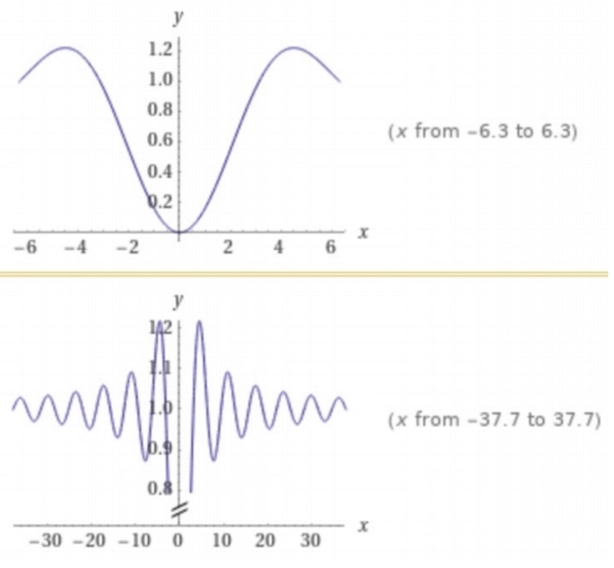
\includegraphics[scale=0.3]{bild.jpg}
							\end{center}
							\end{figure}
						
							Now define 
						 $$\alpha \coloneqq \inf \{ h(x) \colon \lvert x \rvert \geq 1 \} = 1 -\sin(1) > 0$$ so that $\frac{h(x)}{\alpha}\geq 1$ for $|x|>1$. Then, for $k\geq 1$,
		\begin{align*}
			\mu_n \big( [-k,k]^c \big) \overset{\text{mon.}}&{\leq} \int_{[-k,k]^c} \frac{1}{\alpha} h \Big( \frac{x}{k} \Big) \dint \mu_n(x) \\
			&\leq \frac{1}{\alpha} \int_{\mathbb{R}} h \Big( \frac{x}{k} \Big) \dint \mu_n(x) \\
			&= \frac{1}{\alpha} \int_{\mathbb{R}} \underbrace{\bigg( \int_0^1 \Big( 1 - \cos \Big( \frac{t x}{k}\Big) \Big) \dint t \bigg)}_{=1- \sin(\frac{x}{k}) \frac{k}{x} = h(\frac{x}{k})} \dint \mu_n(x) \\
			\overset{\text{Fubini}}&{=} \frac{1}{\alpha} \int_0^1 \int_{\mathbb{R}} \Big( 1 - \cos \Big( \frac{t x}{k} \Big) \Big) \dint \mu_n(x) \dint t \\
			&= \frac{1}{\alpha} \int_0^1 \Big( 1  - \cR e \Big( \varphi_{\mu_n} \Big( \frac{t}{k} \Big) \Big) \Big) \dint t.
		\end{align*}	
						Now we use dominated convergence to obtain
						\begin{align*}
							\limsup_{n\to\infty} \mu_n \big( [-k,k]^c \big) &\leq \frac{1}{\alpha} \lim_{n\to\infty} \int_0^1 \Big( 1 - \cR e \Big( \varphi_{\mu_n} \Big( \frac{t}{k} \Big) \Big) \big) \dint t \\
						\overset{\text{DCT}}&{=} \frac{1}{\alpha} \int_0^1 \lim_{n \to \infty}  \bigg( 1 - \cR e \Big( \varphi_{\mu_n} \Big( \frac{t}{k} \Big) \Big) \bigg) \dint t \\
							&= \frac{1}{\alpha} \int_0^1  \Big( 1 - \cR e \Big( f \Big( \frac{t}{k} \Big) \Big) \Big)
						\end{align*}	
						In the last step we have used that convergence of a sequence of complex numbers implies convergence of real- and imaginary-parts.			
						Finally, we use the continuity of $f$ (and thus $\cR e(f)$) at $0$. For all $\varepsilon > 0$ there is a $\delta>0$ such that $\lvert 0 - \frac{t}{k} \rvert < \delta$ implies $\lvert 1 - \cR e ( f(\frac{t}{k})) ) \rvert = \lvert \cR e(f(0)) - \cR e ( f(\frac{t}{k})) ) \rvert \leq \varepsilon$. Hence, there is some $k$ so that $\lvert 1 - \cR e ( f(\frac{t}{k})) ) \rvert < \varepsilon$ for all $t \in [0,1]$. But then there is some $k$ so that $\limsup_{n\to\infty} \mu_n \big( [-k,k]^c \big) < \varepsilon$. 
				
						From this the tightness follows as every single probability measure on $\mathbb{R}^d$ is tight. ARGUMENT HINSCHREIBEN
	\end{proof}
	%\begin{lsuperwichtigersatz}
	%\begin{corollary}[L\'{e}vy continuity theorem - special formulation]\label{levy_special}
	
	%	\begin{enumerate}[label=(\roman*)]
	%		\item		Suppose $\mu,\mu_1,...\in \cM_1(\mathbb{R}^d)$, then
	%		\begin{align*}
	%			\mu_n \overset{\text{(w)}}{\longrightarrow} \mu,\: n \to \infty \quad\Leftrightarrow \quad \varphi_{\mu_n} \to \varphi_\mu(t),\: n \to \infty,  \quad \forall t \in \mathbb{R}.
	%		\end{align*}
	%		\item Suppose $X,X_1,...$ are $\R^d$-valued random variables, then
	%			\begin{align*}
	%			X_n \overset{\text{(d)}}{\longrightarrow} X, \: n \to \infty \quad \Leftrightarrow \quad \varphi_X(t) \to \varphi_X(t),\: n \to \infty, \quad \forall t \in \mathbb{R}.
	%		\end{align*}				
	%	\end{enumerate}
	%\end{corollary}			
%\end{lsuperwichtigersatz}

We finish the section with a short discussion of the usefulness of the generalised version of the continuity theorem. Let us recall the different ways of characterising random variables: 
\begin{align*}
	\text{random variable }X\quad \Leftrightarrow \quad \text{ law }\P_X\quad \Leftrightarrow \quad \text{CDF }F_X.
\end{align*}
In fact, just as CDFs are functions with a set of properties one can ask if also characteristic functions are functions with a set of axiomatic properties so that it is reasonable to extend 
\begin{align*}
	\text{random variable }X\quad \Leftrightarrow \quad \text{ law }\P_X\quad \Leftrightarrow \quad \text{CDF }F_X\quad \Leftrightarrow\quad \text{characteristic function }\varphi_X.
\end{align*}
Indeed, this is the case but unfortunately the appearing property of positive definitness is hard to check:
\begin{lsatz}
\begin{theorem}[Bochner]
	A function $\varphi \colon \mathbb{R}^d \to \mathbb{C}$ is the characteristic function of a random vector (or a probability measure on $\mathcal B(\R^d)$) if and only if 
	\begin{itemize}
		\item $\varphi(0)=1$
		\item $\varphi$ is continuous at $0$
		\item $\varphi$ is \textbf{positive semidefinite}, i.e. 
		\begin{align*}
			\sum_{k,l=1}^{n} y_k \bar{y}_l \varphi(t_k - t_l) \geq 0, \quad \forall n \in \mathbb{N}, \: t_i \in \mathbb{R}^d, \: y_i \in \mathbb{C}.
		\end{align*}	
	\end{itemize}
\end{theorem}
\end{lsatz}
\begin{proof}[Proof]
	"$\Rightarrow$": Suppose $\varphi(t)=\E[e^{itX}]$ for some random variable $X$. Then $\varphi(0) = 1$ is clear, continuity at $0$ follows from dominated convergence, and
		\begin{align*}
			\sum_{k,l=1} y_k \bar{y}_l \varphi (t_k - t_l) &= \sum_{k,l=1} y_k \bar{y}_l \int_{\mathbb{R}^d} e^{i \langle x, t_k - t_l \rangle} \dint \mu(x) \\
				&= \int_{\mathbb{R}^d} \sum_{k,l=1}^n y_k e^{i \langle x ,t_k \rangle} \overline{y_l e^{i \langle x ,t_l \rangle}} \dint \mu(x) \\
				&= \int_{\mathbb{R}^d} \Big\lvert \sum_{k=1} y_k e^{i \langle x , t_k \rangle} \Big\rvert^2 \dint \mu(x) \geq 0.
		\end{align*}
	"$\Leftarrow$": Too hard
\end{proof}
There are many classes of characteristic functions that can be understood more directly using the general version of the continuity theorem. If for some reason we have a sequence of characteristic functions $\varphi_n$ that converges pointwise to a function $\varphi$ that is continuous at $0$, then $\varphi$ is a characteristic function. For all even continuous functions $\varphi \colon \mathbb{R} \to [0,1]$ with $\varphi(0)=1$ that are convex on $[0,\infty)$ this can be done (P\'olya's theorem). One can in fact construct simple explicit random variables which characteristic functions $\varphi_n$ that are  approximations of such such functions and converge pointwise to $\varphi$.

\begin{figure}[h]
	\begin{center}
		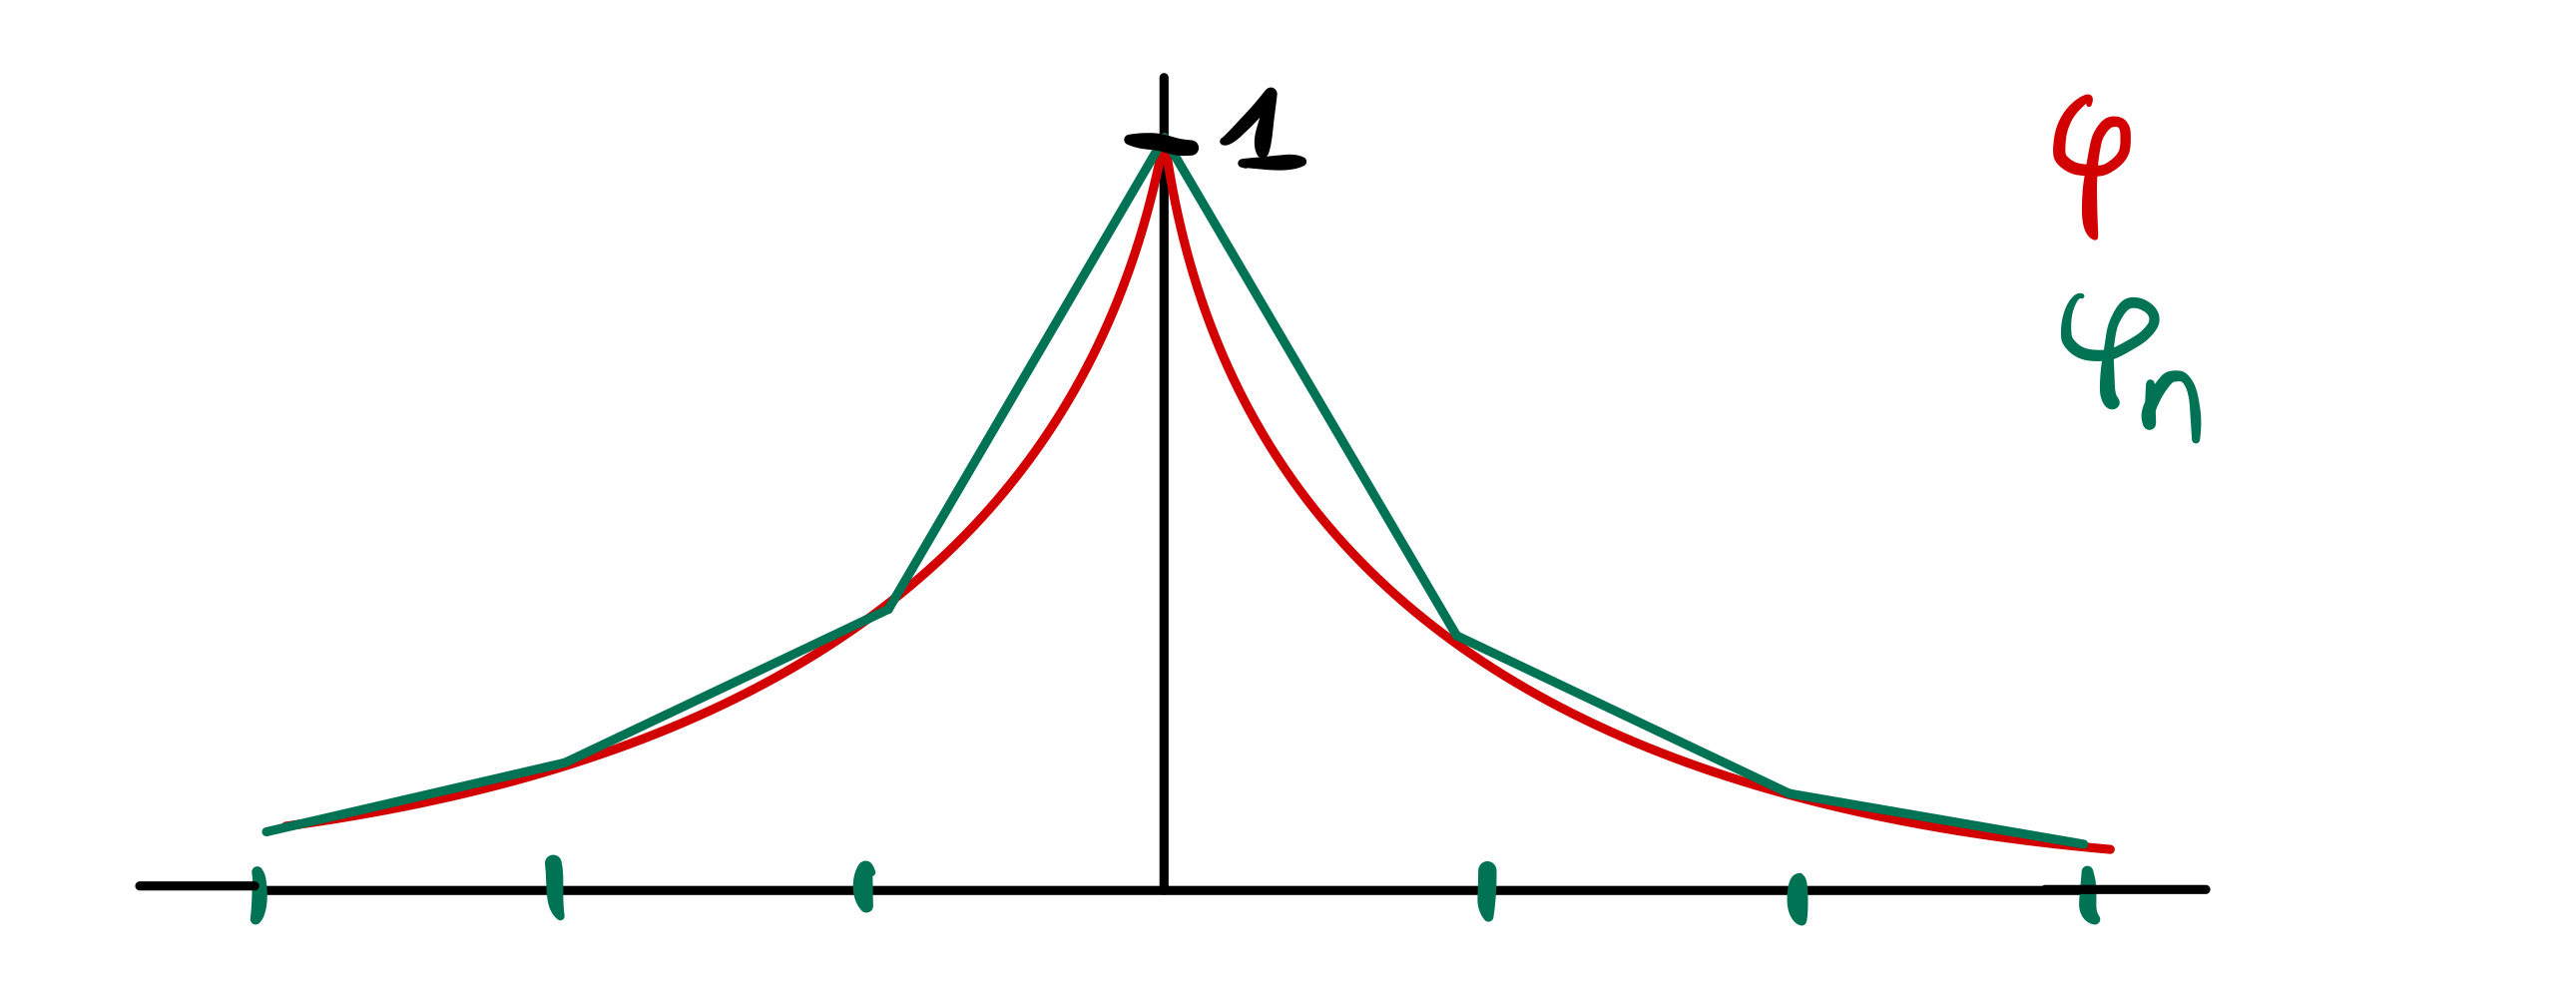
\includegraphics[scale=0.07]{characteristic.jpeg}
	\end{center}
	\vspace{-9mm}
	\end{figure}



\begin{example}
	For $\alpha\in (0,1)$ and $\lambda>0$ the function $\varphi_{\alpha}(t) = e^{- \lambda \lvert t \rvert^{\alpha}}$ is even and convex on $[0,\infty)$. By P\'olya's theorem this is a characteristic function of a random variable $X$. The random variable is called $\alpha$-stable. In fact, the assumption $\alpha\in (0,1)$ is only needed to apply P\'olya's theorem, actually $\varphi_\alpha$ is a characteristic function if and only if $\alpha\in [0,2]$. All such random variables are called $\alpha$-stable and generalise the Gaussian distribution which appears for $\alpha=2$.
\end{example}


	\marginpar{\textcolor{red}{Lecture 18}}



\section{Applications}
Recall from Theorem \ref{erzeugende} the relation $\E[X^n]=\frac{\mathcal M_X^{(n)}(0)}{n!}$ between derivatives of the moment generating function $\mathcal M_X(t)=\E[e^{tX}]$ and the moments. The relation is useful as it allows to compute moments easily for a couple of examples (such as the Gaussian). In principle the idea is very simple, here for the first moment: $$\mathcal M'_X(t)=\frac{d}{dt}\E[e^{tX}]=\E\Big[\frac{d}{dt}e^{tX}\Big]=\E[X e^{tX}]$$ and then plugging-in $t=0$. What makes the proof tricky is the interchange of differentiation and expectation for which dominated convergence needs to be applied in the right way and this forced us to assume finiteness of $\mathcal M_X$ in some interval $(-\varepsilon, \varepsilon)$. Since finiteness of $\mathcal M_X(t)$ means existence of exponential moments the theorem looks much better than it is, the assumption is extremely strong! We will now repeat the same story using the complex exponential. Before doing so we should first say a word on differentiation for functions $f:\R\to \C$. This is either defined by interpreting $\C$ as $\R^2$ and then the rewriting the derivative (a vector) in terms of polar coordinates or directly by taking limits in $\C$: $\frac{d}{dt} f(t)=f'(t)=\lim_{h\to 0}\frac{f(t+h)-f(t)}{h}$. Writing 
\begin{align*}
	\lim_{h\to 0}\frac{f(t+h)-f(t)}{h}=\lim_{h\to 0}\frac{\mathcal R ef(t+h)-\mathcal R ef(t)}{h}+i\lim_{h\to 0}\frac{\mathcal I m f(t+h)-\mathcal I mf(t)}{h}
\end{align*}
shows that both approaches give exactly the same. As always it is important to keep in mind that we can freely ignore the formal definition and just compute in $\C$ as we are used to in $\R$ with the convention $i^2=-1$. Most importantly, it holds that $\frac{d}{dt} e^{itx}=ix e^{itx}$. Higher order derivatives are definded recursively and denoted as usually by $f^{(n)}$. Now suppose, as for moment generating functions, the differentiation can be switched into the expectation, then we should get $\varphi_X^{(n)}(t) = \E \big[ i^n X^ne^{itX} \big]$ so that plugging-in $t=0$ gives again a moment formula $\E[X^n]=\frac{\varphi_X^{(n)}(0)}{i^n}$. Here again the magic of the complex exponential occurs. It is equally powerful in terms of what one can get from it but it is much more friendly because it is bounded. In essense the following theorem shows how to replace the real-exponential (moment generating function) by the complex-exponential (characteristic function) to obtain the same kind of results with minimal assumptions on the random variable.
\begin{lsatz}
\begin{theorem}[Moments of $X$ and differentiability of $\varphi_X$]\label{theorem_moments}
	Let $X$ be a real-valued random variable with characteristic function $\varphi_X$.
	\begin{enumerate}[label=(\roman*)]
		\item
			If $\E[ \lvert X^n \rvert ] < \infty$, then $\varphi_X$ is $n$-times continuously differentiable with $$ \varphi_X^{(n)}(t) = \E \big[ e^{itX}i^n X^n \big], \quad t \in \mathbb{R}.$$
			In particular, $\E[X^n]=\frac{\varphi^{(n)}_X(0)}{i^n }$.
		\item
			If $\E [ \lvert X^n \rvert ] < \infty$ for some $n\in\N$, then $\varphi_X$ satisfies the Taylor approximation
			\begin{align}\label{Taylor}
				\varphi_X(t) = \sum_{k=0}^n \frac{i^k \E[X^k]}{k!} t^k + h_n(t)t^2, \quad t\in \mathbb{R},
			\end{align}
			with a residual term satisfying $\lim\limits_{t \to 0} h_n(t) =0$.
		\item
			If $\lim\limits_{k \to \infty} \frac{t^k \cdot \E [ \lvert X^k \rvert ]}{k!} = 0$ for some $t\in\R$, then $\lim_{n\to\infty} h_n(t) =0$. In particular, $\varphi_X$ has the power series representation
			\begin{align*}
				\varphi_X(t) = \sum_{k=0}^{\infty} \frac{i^k \E[X^k]}{k!}t^k,\quad t\in\R.
			\end{align*}
	\end{enumerate}
\end{theorem}
\end{lsatz}
The power series representation of $\varphi_X$ is not surprsing at all. Writing the complex exponential as a power series and exchanging freely expectation and infinite sum this nothing but
\begin{align*}
	\varphi_X(t)=\E\Big[\sum_{k=0}^\infty \frac{i^kt^kX^k}{k!}\Big]=\sum_{k=0}^\infty \frac{i^k\E[X^k]}{k!}t^k.
\end{align*}
Of course, the interchange is non-trivial and there are essentially two ways to go. Either, arguing as in the proof of Theorem \ref{erzeugende} one takes the limit of the partial sums, justifies dominated convergence, and then gets the moment formual by differentiating the power series, or, as we argue below, one first identifies the derivatives and then refers to Taylor's theorem to derive the power series.
\begin{proof}[Proof]
	In order to swich differentiation and expectation we will use the differential quotient and use dominated convergence to justify the change of expectation and limit in $\varepsilon$. We can do this since the differences of complex exponentials have useful bounds. Let us first check the basic estimate  $\lvert e^{itx} - e^{isx} \rvert \leq \lvert t - s \rvert \cdot \lvert x \rvert $. If $s < t$ and $x > 0$, then expanding the exponential and using the Euler formula yields
	\begin{align*}
		\lvert e^{itx} - e^{isx} \rvert &= \lvert e^{is\frac{x}{2}} \rvert \cdot \lvert e^{it\frac{x}{2}} \rvert \cdot \lvert  e^{i(t-s)\frac{x}{2}} - e^{-i(t-s)\frac{x}{2}} \rvert \\
		&= 2 \lvert \sin ((t-s) x/2 ) \rvert \\
		&= 2  \Big\lvert \int_0^{(t-s) \frac{x}{2}} \cos(u)\dint u \Big\rvert
		\overset{|\cos|\leq 1}{\leq} |(t-s)x|
	\end{align*}
	and the other cases are treated similarly.\smallskip
	
	(i) The first derivative is now simple:
			\begin{align*}
				\lim\limits_{h\to 0} \frac{\varphi_X(t)-\varphi_X(t+h)}{h} = \lim\limits_{h \to 0} \E \bigg[ \frac{e^{itx}-e^{i(t+h)x}}{h} \bigg] 
							\overset{\text{DCT}}{=} \E \bigg[ \lim\limits_{h \to 0} \frac{e^{itx}-e^{i(t+h)x}}{h} \bigg] 
							= \E \big[ i  X  e^{itX} \big]
			\end{align*}
			Changing limits and expectation was justified by the integrable (assumption) upper bound
			\begin{align*}
				\bigg\lvert  \frac{e^{itx}-e^{i(t+h)x}}{h} \bigg\rvert  \leq \frac{\lvert h \cdot x \rvert }{\lvert h \rvert} = \lvert x \rvert
			\end{align*}
			which was justified above. Hence, $\varphi_X^{\prime}(t) = \E \big[ e^{itX}i X \big]$ exists. Inductively we proceed in exactly the same way to differentiate $\varphi_X^{(k)}(t)$:
			\begin{align*}
				\lim_{h\to 0} \frac{\varphi_X^{(k)}(t) - \varphi_X^{(k)}(t+h)}{h} &= \lim_{h\to 0} \frac{\E \big[e^{itX}i^k X^k\big] - \E \big[ e^{i(t+h)X}i^k X^k\big]}{h} \\
			&=\lim_{h\to 0} \E \bigg[ \frac{\big( e^{itX - e^{i(t+h)X}}\big) i^k X^k}{h} \bigg] \\
				\overset{\text{DCT}}&{=} \E \bigg[ \lim_{h\to 0} \frac{\big( e^{itX - e^{i(t+h)X}}\big) i^k X^k}{h} \bigg] 
				= \E \big[ i^{k+1} X^{k+1} e^{itX} \big]
			\end{align*}
			The interchange of limit and expectation is again justified by the upper bound
			\begin{align*}
				\frac{\lvert (e^{itx} - e^{i(t+h)x}) i^k x^k \rvert}{h} \leq \lvert x \rvert \cdot \lvert x^k \rvert = \lvert x^{k+1} \rvert.
			\end{align*}
			The proof shows very clearly that $\varphi_X$ can be differentiated as long as there are enough finite moments of $X$. But this is no additional assumption as otherwise the formula does not make sense anyways!\smallskip

	(ii) Since all derivatives at $0$ are known from (i) the complex version of Taylor's theorem for $x_0 =0$ gives
			\begin{align*}
				\varphi_X(t) = 1+  i t \E[X] - \frac{1}{2} t^2 \E [ X^2] + ... + \frac{i^n t^n\E [X^n]}{n!} + R_n(t)t^n,
			\end{align*}
			with a remainder term satisfying $\lim\limits_{t\to 0} h_n(t) = 0$.\smallskip

	(iii)
			We need to show that, for fixed $t$, the residual $h_n(t)$ vanishes as $n$ tends to infinity. It is most practical to use the integral representation for $R_n(t):=h_n(t)t^n$:
			\begin{align*}
				\lvert R_n(t) \rvert = \Big\lvert \int_0^t \frac{\varphi_X^{(n+1)}(s)}{(n+1)!}(t-s)^n \dint s \Big\rvert &\leq \int_0^t \frac{\E [ \lvert X^{n+1}\rvert] }{(n+1)!}(t-s)^n \dint s
				 = \frac{t^{n+1}}{(n+1)} \frac{\E[ \lvert X^{n+1}\rvert ]}{(n+1)!}
			\end{align*}
			Here we used the formula from (i) and that $|e^{itX}i^n|=1$. But then $h_n(t)\to 0$ for $n\to\infty$.
\end{proof}
Just as we used the moment generating functions to compute moments for random variables with exponential moments we can also use the characteristic functions:
\begin{luebung}
	Compute the first few moments of $\mathcal N(0,1)$, $\text{Poi}(\lambda)$, and $\mathcal U([0,1])$.
\end{luebung}
As an application we prove what is sometimes called the \textbf{method of moments} and, as a special case, we can finally give a proof of Theorem \ref{WT}.
\begin{llemma}
\begin{corollary}
	\begin{enumerate}[label=(\roman*)]
		\item
			Let $X$ be a real-valued random variable such that there is a constant $C$ with $\frac{1}{n} \big( \E[\lvert X^n \rvert ] \big)^{\frac{1}{n}}< C$ for all $n\in \mathbb{N}$. Then the law of $X$ is uniquely determined by all it's moments.
		\item
			In particular, if $\mathcal M_X(t) < \infty$ for $t \in (-\varepsilon,\varepsilon)$ for some $\varepsilon > 0$, then $\mathcal M_X$ uniquely determines the law of $X$.
	\end{enumerate}
\end{corollary}
\end{llemma}
The corollary is a significant extension of Theorem \ref{coruniq}. If $|X|$ is bounded by some $C$, then $\E[|X^n|]$ is bounded by $C^n$ so that the assumption of the corollary is clearly satisfied. The corollary states that also for other (rather special) random variables which moments increase slowly enough the same statement holds.
\begin{proof}[Proof]
			(i) For $\lvert t \rvert < \frac{1}{3C}$ we have
			\begin{align*}
				\limsup_{n\to \infty} \frac{\E [ \lvert X^n \rvert ] \cdot \lvert t \rvert^n}{n!} \overset{\text{Sterling}}&{=} \limsup_{n\to \infty} \Big( \E [ \lvert X^n \rvert ]^{\frac{1}{n}}  \lvert t \rvert  \frac{e}{n} \Big)^n  \sqrt{2 \pi n}
					\leq \limsup_{n\to \infty} \Big( \frac{e}{3} \Big)^n \sqrt{2\pi n}
					= 0
			\end{align*}
			Hence, for all $t \in (-\frac{1}{3C}, \frac{1}{3C})$ we can use Theorem \ref{theorem_moments} (iii) to express $\varphi_X$ as a power series. Since the coefficients are the moments, $\varphi_X$ is determined on $(-\frac{1}{3C},\frac{1}{3C})$ through the moments. Since a power series is uniquely determined by the values on some interval $\varphi_X$ is also uniquely determined on $\R$ by all the moments. Finally, since the law of $X$ is uniquely determined by $\varphi_X$ according to Theorem \ref{CF} the proof is complete.\smallskip

			(ii) We argue as in the proof of Theorem \ref{erzeugende}:
			\begin{align*}
				\sum_{k=0}^{\infty} \frac{t^k \E[ \lvert X \rvert^k]}{k!} \overset{\text{MCT}}=  \E [ e^{t\lvert X \rvert}]\leq \E[e^{tX}]+\E[e^{-tX}]=\mathcal M_X(t)+\mathcal M_X(-t)<\infty,\quad t\in (-\varepsilon, \varepsilon).
			\end{align*}	
			Now we can use the proof of (i) to finish the proof.	
\end{proof}
\begin{lsuperwichtigersatz}
	\begin{theorem}[Central Limit Theorem]
	Let $X_1,X_2,...$ be iid with $\mu \coloneqq \E[ X_1]$ and $\sigma^2 \coloneqq \mathbb{V}[X_1] < \infty$. Then
	\begin{align*}
		\frac{\sum_{k=1}^n X_k - n \mu}{\sqrt{\sigma^2 n}} \overset{\text{(d)}}{\longrightarrow} \cN(0,1), \quad n \to \infty.
	\end{align*}
\end{theorem}
\end{lsuperwichtigersatz}

\begin{proof}[Proof]
	Without loss of generality we may assume $\mu=0$ and $\sigma^2=1$ as otherwise we can consider the standardised random variables $\tilde{X} \coloneqq \frac{X-\mu}{\sigma}$. Writing $S_n=\sum_{k=1}^n X_k$, L\'{e}vy's continuity theorem we only need to prove that
	\begin{align*}
		\varphi_{\frac{S_n}{\sqrt{n}}}(t) \longrightarrow e^{-\frac{1}{2}t^2} = \varphi_{\cN(0,1)}(t),\quad \forall t \in \mathbb{R}.
	\end{align*}
	Using Lemma \ref{lemma_5111} and the iid assumption shows that we only need to prove
	\begin{align*}
		\varphi_{\frac{S_n}{\sqrt{n}}}(t) = \Big( \varphi_{X_1}\Big( \frac{t}{\sqrt{n}}\Big) \Big)^n \longrightarrow e^{-\frac{1}{2}t^2}, \quad n \to \infty.
	\end{align*}	
The trick is to replace the exponential by the first two summands of it's Taylor expansion \eqref{Taylor} and then to use
\begin{align*}
	\lim_{n\to\infty}\Big(1-  \frac{t^2}{2n}\Big)^{n}= e^{-\frac{1}{2}t^2},\quad t\in\R.
\end{align*}
Do do this rigorously first check by a quick induction that
	\begin{align*}
		\lvert u^n - v^n \rvert \leq \lvert u - v \rvert \cdot n \cdot \max(\lvert u \rvert, \lvert v \rvert )^{n-1}, \quad\forall u,v\in\mathbb{C}.
	\end{align*}
	Using that $|\varphi_{X_1}|, |1 - \frac{t^2}{2n}|\leq 1$ for $n$ large enough then yields
	\begin{align*}
		\bigg\lvert \Big( 1 - \frac{t^2}{2n} \Big)^n - \Big(\varphi_{ X_1}\big(\frac{t}{\sqrt{n}}\big)\Big)^n \bigg\rvert 
		&\leq \bigg\lvert \Big( 1 - \frac{t^2}{2n} \Big)^n - \Big( 1 - \frac{1}{2} \frac{t^2}{n} + h_2\Big( \frac{t}{\sqrt{n}} \Big) \frac{t^2}{n} \Big)^n \bigg\rvert \\
		&\leq n \cdot \Big\lvert h_2 \Big( \frac{t}{\sqrt{n}}\Big)  \frac{t^2}{n} \Big\rvert \\
		&= t^2 \cdot \Big\lvert h_2 \Big( \frac{t}{\sqrt{n}} \Big) \Big\rvert
		\rightarrow 0,\quad n \to \infty.
	\end{align*}
\end{proof}
In many textbooks one can see the formulation
	\begin{align*}
		\lim_{n\to\infty}\mathbb{P} \bigg( \frac{\sum_{k=0}^n X_k - n \cdot \mu}{\sqrt{n \sigma^2}} \in [a,b] \bigg)= \frac{1}{\sqrt{2\pi}} \int_a^b e^{- \frac{x^2}{2}} \dint x, \quad \forall a<b,
	\end{align*}
	which holds due to Portemanteau because $\mathbb{P}_{\cN(0,1)}( \partial [a,b]) = 0$.


\chapter{Brownian Motion}\label{sec:BM}

